% Template for the submittion to:
%   The Annals of Probability           [aop]
%   The Annals of Applied Probability   [aap]
%   The Annals of Statistics            [aos]
%
%Author: In this template, the places where you need to add information
%        (or delete line) are indicated by {???}.  Mostly the information
%        required is obvious, but some explanations are given in lines starting
%Author:
%All other lines should be ignored.  After editing, there should be
%no instances of ??? after this line.

% use option [preprint] to remove info line at bottom
% journal options: aop,aap,aos
%\documentclass[aos]{imsart}
\documentclass{imsart}

\usepackage{amsthm,amsmath,natbib}
%\RequirePackage[dvips]{hyperref}

% use this package if hyperref and natbib is used:
%\RequirePackage{hypernat}

% provide arXiv number if available:
%\arxiv{math.PR/0000000}

% put your definitions there:
\startlocaldefs
\usepackage{algorithm}
\usepackage{algorithmic,amssymb}
\usepackage{graphicx,xcolor}
\usepackage{subfigure}
%\usepackage[boxed]{algorithm2e}


\renewcommand{\algorithmicrequire}{\textbf{Input:}}
\renewcommand{\algorithmicensure}{\textbf{Output:}}
\renewcommand{\algorithmiccomment}[1]{\# #1}

\newcommand{\argmax}{\mathop{\mathrm{argmax}}}
\newcommand{\argmin}{\mathop{\mathrm{argmin}}}
\newcommand{\minimize}{\mathop{\mathrm{minimize}}}
\newcommand{\maximize}{\mathop{\mathrm{maximize}}}

\newcommand{\todo}{\textcolor{red}{\textbf{To do: }}}

\newcommand{\real}{\mathbb{R}}
\newcommand{\Pp}{{\mathbb P}}
\newcommand{\Ee}{{\mathbb E}}
\newcommand{\lips}{{\cal L}}
\newcommand{\tube}{\mathrm{Tube}}
\newcommand{\sphere}[1]{O^{#1-1}}
\newcommand{\dimens}{\text{dim}}
\newcommand{\cone}{\text{Cone}}
\newtheorem{theorem}{Theorem}
\newtheorem{lemma}[theorem]{Lemma}
\newtheorem{cor}[theorem]{Corollary}
\newcommand{\XK}{K_X}
\newcommand{\norm}[1]{\lVert #1 \rVert}
\newcommand{\innerp}[2]{\langle #1 , #2 \rangle}
%\newcommand{\qed}{\hfill $\Box$\newline}

\newcommand{\grad}{\nabla}
\newcommand{\V}{\mathcal{V}}\endlocaldefs
\newcommand{\K}{\mathcal{K}}
\newcommand\tf{\widetilde{f}}
\newcommand{\pen}{\mathcal{P}}
\newcommand{\vecsp}{\mathcal{L}}
\newcommand{\gstar}{g^*}

\newcommand{\jonathan}[1]{{\color{blue}  #1}}
\newcommand{\josh}[1]{{\color{green} #1}}

\begin{document}

\begin{frontmatter}

% "Title of the paper"
\title{A significance test in forward stepwise model selection}

%%%
%%% \runtitle{} - I don't know what this is
%%%

% indicate corresponding author with \corref{}
%\author{\fnms{Jonathan} \snm{Taylor}\corref{Jonathan E. Taylor}\ead[label=e1]{jonathan.taylor@stanford.edu}\thanksref{t1}
%\and \fnms{Joshua} \snm{Loftus}}
%\thankstext{t1}{Supported in part by NSF grant DMS 1208857 and AFOSR grant 113039.}

\affiliation{Stanford University}

\address{Department of Statistics\\  Stanford University\\ Sequoia
Hall \\390 Serra Mall\\ Stanford, CA 94305, U.S.A.\\ }
%\printead{e1}}

%%%
%%% \runauthor{Taylor} - I don't know what this is
%%%

\begin{abstract}
% perhaps de-emphasize group LASSO and emphasize forward stepwise?
  We extend the methods developed by \cite{significance:lasso} and
  \cite{tests:adaptive} on significance tests for penalized
  regression to stepwise model selection by iteratively applying
  the global null hypothesis test on the residual in a forward stepwise
  procedure. The resulting method
  has the computational strengths of stepwise selection and partially
  solves the problem of inflated test statistics due to model selection.
  In describing our variant of forward stepwise selection, we introduce
  a new class of selection procedures, described by quadratic inequalities and
  provide an algorithm that can be used for exact post-selection inference for such problems.
  
  We illustrate the flexibility of our procedure by applying it to
  novel specialized applications of forward stepwise to a hierarchically
  constrained interactions model and recently described flexible additive models
  that choose between linear and nonlinear effects for each variable.
\end{abstract}

%%%
%%% - Gotta change these??????????
%%%
\begin{keyword}[class=AMS]
\kwd[Primary ]{62M40}
%\kwd{}
\kwd[; secondary ]{62H35}
\end{keyword}

\begin{keyword}
\kwd{forward stepwise}
\kwd{model selection}
\kwd{significance test}
\end{keyword}

\end{frontmatter}


\section{Introduction}
\label{sec:intro}

Consider the regression setting with a single response variable $Y$
and collection of predictor or covariate variables denoted $\mathcal X$.
One often wishes to choose a subset of variables $X \subset \mathcal X$
for modeling the response, assuming the remaining variables are
irrelevent and can be discarded without much loss of predictive
or explanatory power. Doing this in a structured and principled way
usually requires algorithmic methods for choosing $X$. One such method,
forward stepwise regression, is a procedure
that begins with an empty model and sequentially adds the best predictor
variable in each step. Because of the stochastic nature of this
algorithm--making use of the data to choose variables--
the usual $\chi^2$ and $F$-tests for significance
fail when a model has been selected this way and tend to be
anti-conservative unless they are computed on a held-out validation
dataset. This is one instance of the general problem of conducting
inference and model selection using the same data, a problem
of central importance on which some recent progress has been made.

In the LASSO setting, \cite{significance:lasso} derived
a novel test statistic and its asymptotic null distribution, making
possible valid inferences after model selection using the full data.
\cite{tests:adaptive} modified and extended those results to the
group LASSO \citep{grouplasso} and other penalized regression
problems, but only under the global null hypothesis.
One of the strengths of these test statistics is that they can be
used for valid significance testing when computed on the same
data used for model selection, eliminating the need for data splitting
or for situations in which data splitting is not appropriate. For example,
when categorical covariates contain rare levels with very few observations
it can be difficult or impossible to split the sample with an adequate
number of such observations occurring in each split.

The present work iteratively applies the global null test
of \cite{tests:adaptive} for each step in forward stepwise selection,
and works out some of the details necessary for
models with grouped variables. The resulting method can
be more statistically efficient than validation on held-out data, and
more computationally efficient than penalized methods with
regularization parameters chosen by cross-validation.

As a small illustrative example, consider a response $Y$ with ten
categorical predictors $X_g$ having between 2 and 4 levels. The true 
relationship is that $Y$ only depends on $X_1$ and $X_9$. Specifically,
if observation $i$ has covariates $X_{1,i} = j, X_{9,i} = k$ then
\[
    Y_i = \beta_{1,j} + \beta_{9,k} + \epsilon_i , \qquad
    \epsilon_i \sim N(0,1)
\]
$X_1$ has three levels with $\beta_1 = (1, .5, -1)$, $X_9$
has two levels with $\beta_9 = (.5, -.5)$. We generated a random
categorical design matrix $X$ and created an instance of this example
with $n = 40$ observations. Running forward stepwise, we calculated
both our p-value and the usual $\chi^2$ p-value at each step. In
Table~\ref{tab:example} we see that forward stepwise chooses the
truly nonzero variables first and both p-values for these are small.
However, once forward stepwise begins adding noise variables, the
$\chi^2$ p-value remains relatively small, potentially leading to 
incorrect inferences.


% latex table generated in R 3.0.2 by xtable 1.7-1 package
% Tue May 13 15:41:11 2014
\begin{table}[ht]
\centering
\begin{tabular}{l|rrrrrrrr}
  \hline
Step & 1 & 2 & 3 & 4 & 5 & 6 & 7 & 8 \\ 
  \hline
Variable & 1 & 9 & 2 & 8 & 4 & 7 & 3 & 10 \\ 
  \hline
  $T\chi$ & 0.00 & 0.01 & 0.16 & 0.60 & 0.72 & 0.81 & 0.84 & 0.92 \\ 
  $\chi^2$ & 0.00 & 0.00 & 0.04 & 0.21 & 0.29 & 0.56 & 0.73 & 0.82 \\ 
  max-$\chi$ & 0.00 & 0.04 & 0.50 & 0.98 & 0.98 & 0.99 & 0.99 & 0.98 \\ 
   \hline
\end{tabular}
\caption{\em Small comparison of $p$-values. Elapsed time for forward stepwise \textit{and} $T\chi$ computation: 0.022 seconds, and for Monte Carlo sample estimate of max-$\chi$ with $M=200$: 0.235 seconds.} 
\label{tab:example}
\end{table}



In the next section we establish general notation and describe the
forward stepwise algorithm used throughout the paper.
Section~\ref{sec:testing} reviews some recent work on
post-selection inference
\citep{significance:lasso,tests:adaptive,lasso:fixed}
relevant to our work here, and describes a general framework
for post-selection inference based on quadratic comparisons.
Simulation results in Section~\ref{sec:simulations} show
empirically that our method performs well in settings where forward
stepwise itself performs well, and that
various stopping rules using our test statistic--including
some from \cite{sequential:fdr}--appear promising. In
Section~\ref{sec:applications} we apply
the method to several variants of forward
stepwise tailored to models with interactions and generalized additive
models, as well as to a real data example involving genomic prediction
of individual drug responses to treat HIV.

%%%%%%%%%%%%%%%%%%%%%%%%%%%%%%%%%%%%%%%%%%%%%%%%%%%%
%%%%%%%%%%%%%%%%%%%%%%%%%%%%%%%%%%%%%%%%%%%%%%%%%%%%
%%%%%%%%%%%%%%%%%%%%%%%%%%%%%%%%%%%%%%%%%%%%%%%%%%%%

\section{Forward stepwise model selection}
\label{sec:stepwise}

\subsection{Background and notation}

\begin{figure}
\begin{center}
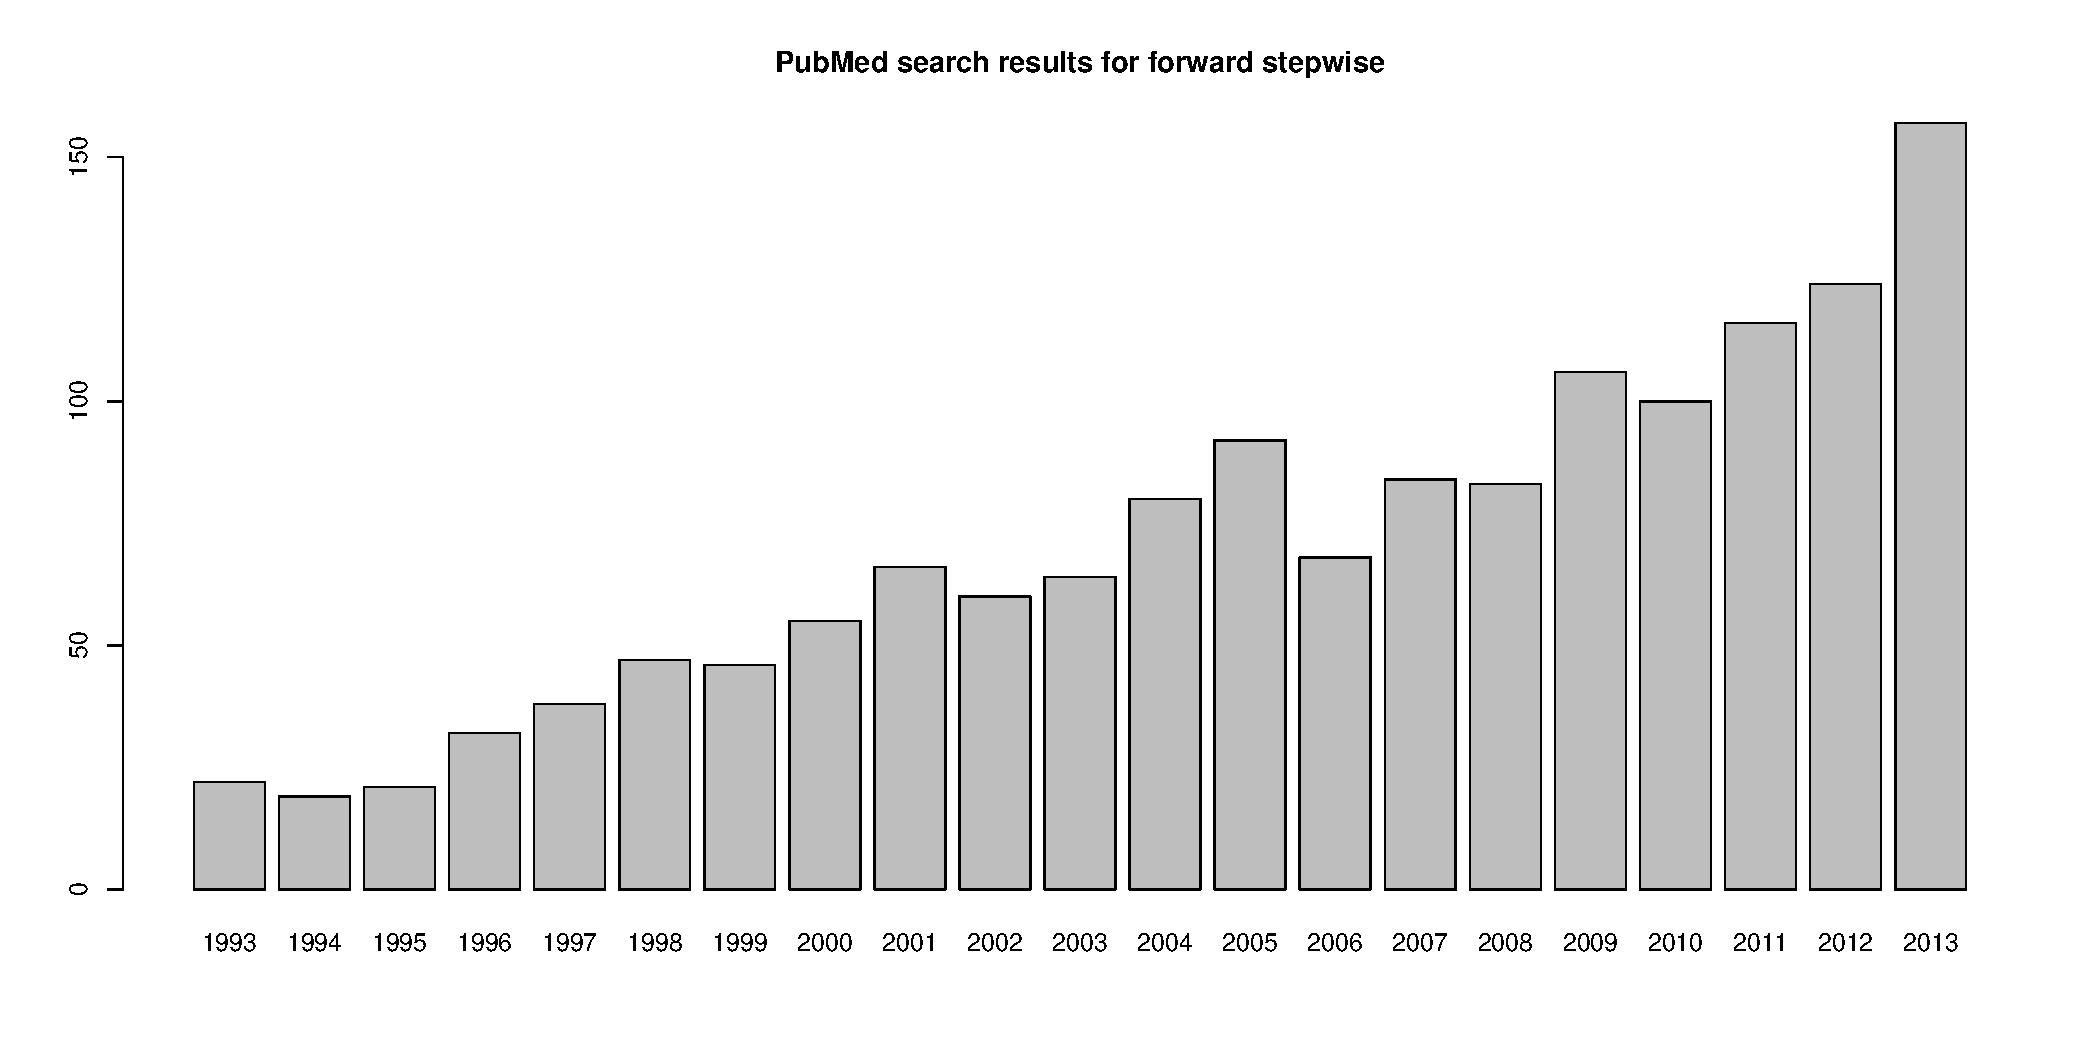
\includegraphics[width=0.9\textwidth]{../figs/pubmed.pdf}
\caption{\small \it Forward stepwise enjoys widespread use among
practitioners}
\label{fig:pubmed}
\end{center}
\end{figure}


As a classical method dating back about half a century
(see \cite{classical:selection} for a review),
forward stepwise regression has not received much attention in
recent years in the theoretical statistics community. But it continues
to be widely used by practitioners.
For example, search results on PubMed for forward stepwise,
summarized in Figure~\ref{fig:pubmed}, show that many recent
papers mention the method and there is an increasing trend over time.
Its popularity among researchers continues despite the fact that it
invalidates inferences using the standard $\chi^2$ or $F$-tests.


Some attempts to address this issue include Monte Carlo
estimation of tables of adjusted $F$-statistic values \citep{mc:ftoenter},
and permutation statistics \citep{permutation:stop}. Aside from the works
this paper is based on, there have been other recent attempts to do
inference after model selection. Most of these make use of subsampling
\citep{meinshausen:buhlmann} or data splitting \citep{wasserman:roeder}.
Our approach allows use of the full data and does not require the
extra computation involved in subsampling.
Before describing the full approach we first introduce notation and
specify our implementation of forward stepwise, which is slightly
different from the most commonly used versions.


We allow forward stepwise selection to add groups of variables in each
step, not only in the case of dummy variable encoding for categorical
variables but also for any grouping purpose. For example, groups of
variables may be pre-designated factors such as expression
measurements for all genes in a single functional pathway.
To emphasize this we use $g, h$ as covariate indices rather than the usual
$i, j$ throughout. Since single variables can be considered groups of
size 1, this includes non-grouped situations as a special
case. Our variant of forward stepwise uses a different method than
usual for choosing which group to add because we are using the
same objective in the forward stepwise procedure that was used to
derive the test statistics in penalized regression settings.

Denote $y \in \real^n$ for $n$ i.i.d. measurements of the outcome variable.
Let an integer $G \geq 2$ be the number of groups of explanatory variables.
For each $1 \leq g \leq G$ the design matrix encoding the
$g$th group is the $n \times p_g$ matrix denoted $X_g$, where $p_g$ is
the number of individual variables or columns in group $g$.
% Do we need to assume $p_g \ll n$ or $\text{rank}(X_g) = p_g$?
When a group encodes a categorical variable as indicators for the
levels of that variable, by default we use the full encoding with a
column for every level. Although this introduces collinearity, our method
does not require the design matrix to have full rank.


Denote $p = \sum_{g=1}^Gp_g$,
the total number of individual variables, so $p = G$ in the
case where all groups have size 1. Let $X$ be the matrix constructed
by column-binding the $X_g$, that is  
%%%%%%%%%%%%%%%%%%%%%%%%%%%%%%%%%%%%%%%%%%%%%%%%
\begin{equation*}
X = \begin{pmatrix} X_1 & X_2 & \cdots & X_G  \end{pmatrix}
\end{equation*}
%%%%%%%%%%%%%%%%%%%%%%%%%%%%%%%%%%%%%%%%%%%%%%%%
We normalize each group by its Frobenius norm, but this is not required
especially since we also allow weights, $w_g$, for each group. These
weights act like penalties or costs, so increasing $w_g$ makes it
more difficult for the group $X_g$ to enter the model. The
modeler can choose weights arbitrarily, but we set them all to be
1 since we already normalize by the Frobenius norm.

With each group we associate the $p_g \times 1$ coefficient vector
$\beta_g$, and write $\beta$ for the $p \times 1$ vector constructed
by stacking all of the $\beta_g$ in order.  Finally, our model for the
response is
%%%%%%%%%%%%%%%%%%%%%%%%%%%%%%%%%%%%%%%%%%%%%%%%
\begin{equation}
\begin{aligned}
\label{eq:gmodel}
y | X& = X \beta + \sigma \epsilon \\
   & = \sum_{g=1}^G X_g \beta_g + \sigma \epsilon
\end{aligned}
\end{equation}
%%%%%%%%%%%%%%%%%%%%%%%%%%%%%%%%%%%%%%%%%%%%%%%%
where $\epsilon$ is noise. We assume Gaussian noise
$\epsilon | X \sim N(0, \Sigma)$ with known covariance matrix $\Sigma$.


The model \eqref{eq:gmodel} is underdetermined when $p > n$.
In such cases it still may be possible to
estimate $\beta$ well if it is sparse--that is, if it has few nonzero
entries. In the rest of this paper we refer to variable groups $X_g$
as noise groups if $\beta_g$ is a zero vector and as true or signal
groups if $\beta_g$ has any nonzero entries. We refer to the number
of such nonzero groups as the \textit{sparsity} of the model, and
denote this $k := \# \{ g : \beta_g \neq 0 \}$. With this notation
we are now ready to describe our procedure concretely.


\subsection{Description of the algorithm}

First, the user must specify the maximum number of steps allowed,
which we denote \textit{steps} (consistent with the \textit{R} function
for stepwise). To enable our test statistic computations,
\textit{steps} should be at most $\min (n, G) - 1$, but it is
computationally desirable to set it as low as possible while
safely larger than the sparsity of $\beta$. 
Then forward stepwise may recover all the nonzero
coefficients of $\beta$ and terminate without performing much
additional computation.
Of course the sparsity is usually unknown, so this requires guesswork.
In our implementation we treat the active set $A$ as an ordered list to easily track the order of groups entering the model.

\begin{algorithm}
  \caption{Forward stepwise variant with groups and weights}
  \label{algo:fs}
  \begin{algorithmic}[1]
    \REQUIRE An $n$ vector $y$ and $n \times p$ matrix $X$ of $G$ variable groups with weights $w_g$
    \ENSURE Ordered active set $A$ of variable groups included in the model at each step
    \STATE $A \gets \emptyset$, $A^c \gets \{ 1, \ldots, G\}$, $r_0 \gets y$
    \FOR{$s=1$ to $steps$}
    \STATE $g^* \gets \argmax_{g \in A^c} \{ \norm{X_g^Tr_{s-1}}_2 / w_g \}$
    \STATE $P_{g^*} \gets I_{n\times n} - X_{g^*}X_{g^*}^\dagger$
    \STATE $A \gets A \cup \{ g^* \}$, $A^c \gets A^c \backslash \{ g^* \}$
    \FORALL{$h \in A^c$}
      \STATE $X_h \gets P_{g^*} X_h$
    \ENDFOR
    \STATE $r_s \gets P_{g^*} r_{s-1}$
    \ENDFOR
    \RETURN $A$
  \end{algorithmic}
\end{algorithm}

The active set $A$ contains variable groups chosen to be included in
the model. Fitting $\hat \beta$ can be done by tracking the individual
fits and projections, or by simply fitting a linear model on the submatrix
of $X$ corresponding to $A$. 
 Note that other
implementations of forward stepwise use different criteria for choosing
the next variable to add, such as the correlation with the residual.
Since we do not renormalize the columns after projecting the covariates
(lines 6 to 8 above), and since we have weights, we are generally not computing
correlations unless the design matrix is orthogonal and all weights are 1. We could
renormalize the columns, though we choose not to.
There are advantages and disadvantages to both criteria which we do not
discuss. Our choice was motivated by the group LASSO result in
\cite{tests:adaptive}, but we believe other criteria can be handled
with appropriate modifications.
We now use forward stepwise to refer specifically to
Algorithm~\ref{algo:fs} unless otherwise specified.

\subsection{Performance of forward stepwise}
\label{sec:fs:performance}

Among model selection procedures, forward stepwise is one which performs
variable selection: from a potentially large set of variables it chooses
a subset to include in the model. The most ambitious form of variable
selection is  ``best-subset'' selection, a procedure which picks the
best model among all $2^G$ subsets of the $G$ possible groups.
This exhaustive search is computationally infeasible when $G$ is
large, and when possible it still
runs the risk of over-fitting unless model complexity is
appropriately penalized (as in \eqref{eq:subsetregress} below).
Forward stepwise produces a much
smaller set of potential models, with cardinality at most
\textit{steps} (which, recall, is less than $\min(n,G)$). However
it is a greedy algorithm, so the set of models it produces may not
contain the best possible model. This is an inherent shortcoming of
forward stepwise procedures and should be kept in mind when choosing
between model selection methods.

So far we have left open the question of choosing among the models in
the forward stepwise sequence, i.e. when to stop stepping
forward. Some approaches for this problem can be posed as optimization
criteria which stop at the step minimizing
\begin{equation}
\begin{aligned}
\label{eq:subsetregress}
\frac{1}{2} \| y - X \beta_s \|_2^2 + \lambda \pen(\beta_s)
\end{aligned}
\end{equation}
where we have written $\{ \beta_s : s = 1, \ldots, steps \}$ as
the sequence of models output by forward stepwise. The function
$\pen(\beta)$ is a penalty on model complexity usually taken to be the
number of nonzero entries of $\beta$. Proposals for $\lambda$ include
2 ($C_p$ of \cite{CP}, AIC of \cite{AIC}), $\log(n)$ (BIC of \cite{BIC}), and
$2\log(p)$ (RIC of \cite{RIC}). Stopping rules based on classical test
statistics have also been used, so it is natural to consider using
the new test statistics of \cite{significance:lasso} or
\cite{tests:adaptive}
to choose a model. \cite{sequential:fdr} examined some stopping rules
using the asymptotic p-values of \cite{significance:lasso} and showed
their stopping rules control false discovery rate--the expected
proportion of noise variables among variables declared significant
\citep{fdr}. We explore this further in Section~\ref{sec:simulations}.

Although forward stepwise is a greedy algorithm producing a
potentially sub-optimal sequence of models, under favorable conditions
it can still perform well. There is a subset of the compressed sensing literature \citep{donoho:pursuit, cai:wang:omp} dedicated to forward stepwise (often referred to in that literature as Orthogonal Matching Pursuit or OMP). 
Typical results from these works establish that forward stepwise can exactly select the true model under some stringent conditions involving quantities like the sparsity of the true model and the coherence of the design matrix.
The coherence $\mu(X)$ of a matrix $X$ with columns scaled to have unit 2-norm is defined as
\begin{equation}
  \mu := \mu(X) = \max_{i \neq j} \{ | \innerp{ X_i }{ X_j } | \}
\end{equation}
Denoting $k$ as the sparsity of $\beta$, the literature establishes
that if $k < (1/\mu + 1)/2$ and the nonzero coefficients of $\beta$ are sufficiently large then forward stepwise recovers $\beta$ with high probability.
The coherence condition is necessary to guarantee exact recovery \citep{cai:wang:xu:sharp} in the sense that it is possible to construct counterexamples with $k = (1/\mu + 1)/2$.
We refer the reader to \cite{donoho:pursuit, cai:wang:omp} for details.
For our purposes the conditions required to guarantee exact recovery are usually too stringent.
Simulations show empirically that forward stepwise can work well even when it is not working perfectly, and that it does so under a wide range of conditions.

\begin{figure}
\begin{center}
\subfigure[Categorical designs]{
\label{fig:fscat}
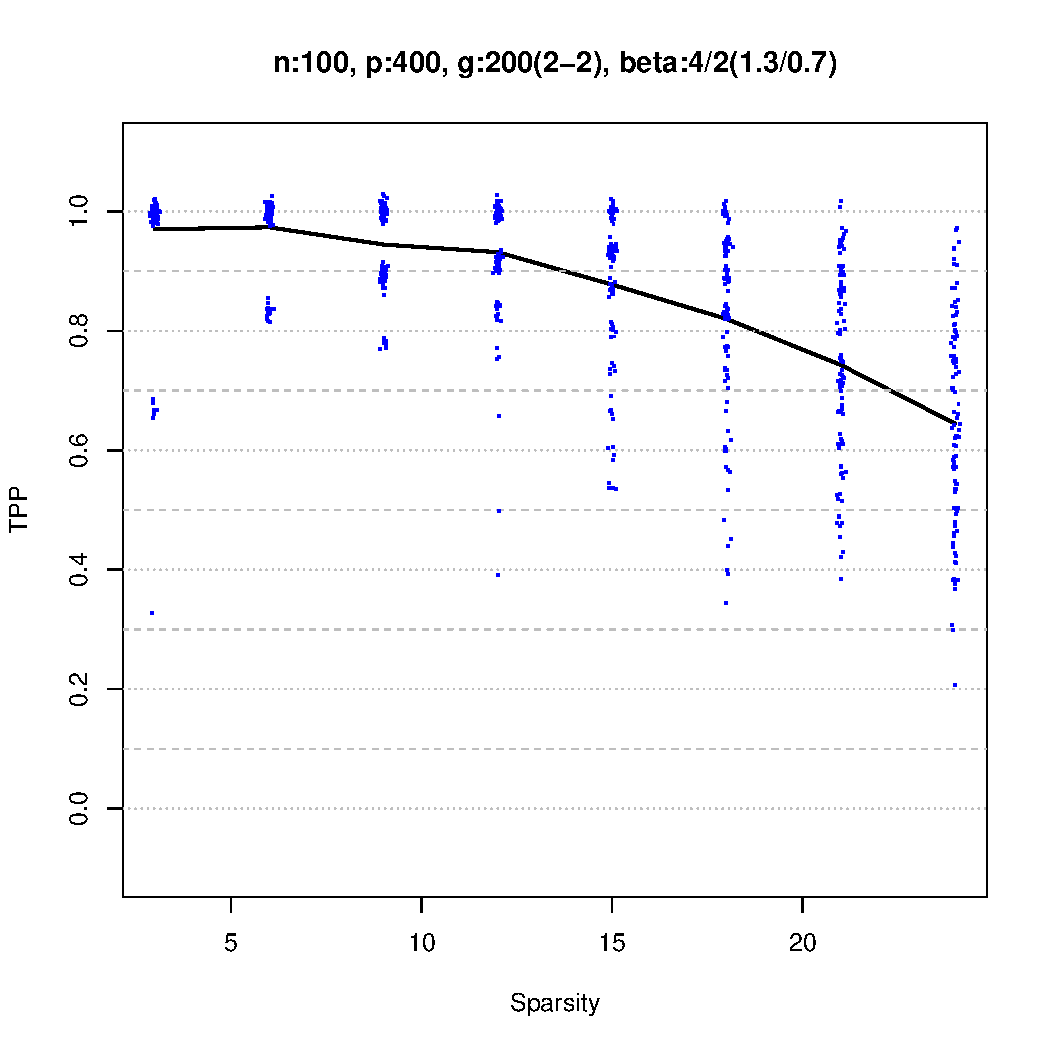
\includegraphics[width=0.5\textwidth]{../figs/tpr_default_categorical_nsim100_n100_p400_g200_sizes2-2_k24_lower2_upper4.pdf}}
\hspace{-15pt}
\subfigure[Gaussian designs]{
\label{fig:fsgausscorr}
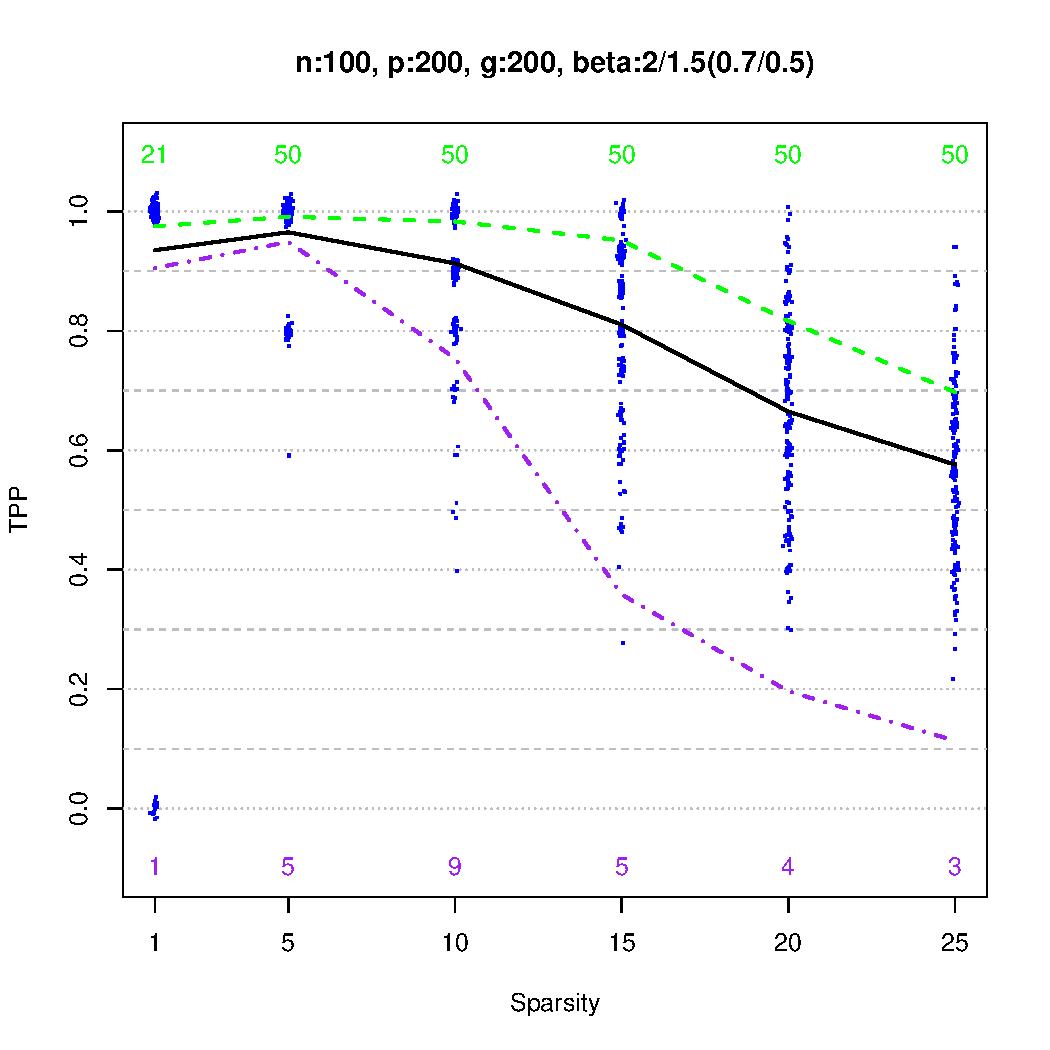
\includegraphics[width=0.5\textwidth]{../figs/tpr_default_gaussian_nsim200_n100_p200_g200_k25_lower1pt5_upper2.pdf}}
\caption{\small \it The left panel shows the results of the simulation
  using a categorical design consisting of 200 binary factors.
  The right panel shows the results with design matrices of Gaussian
  entries. Plotted in green are the TPP (dashed line) and median model
  sizes (top) for models chosen by BIC, and in purple the same are shown
  (dot-dash line, bottom) for RIC.}
\label{fig:fwdstepsim}
\end{center}
\end{figure}

For various sparsity levels $k$, we applied Algorithm~\ref{algo:fs} to
various data sets with \textit{steps} set to $k$.
In the resulting active set $A_k$, the number of true variables divided by $k$ is the $k$-True Positive Proportion ($k$-TPP):
\[
k\text{-TPP} = \frac{\# \left\{g: g \in A_k, \beta_g \neq 0\right\}}{k}.
\]
Since we know $k$ in the simulations we can use $k$-TPP as a measure of how well forward stepwise is performing. When it is close to 1 we are recovering most of the true variables before including false ones.
In our simulations nonzero coefficients have magnitudes
in a range of multiples of $\gamma := \sqrt{2\log(G)/n}$, e.g. in $[1.4
\gamma, 1.6 \gamma]$. Results are shown in
Figure~\ref{fig:fwdstepsim}. After computing the
coherence of these design matrices, some calculations show the required
sparsity level to guarantee exact recovery in these situations is
about 2 or smaller, and the required nonzero coefficient magnitude is
likely in the range of 10 to 100 times $\gamma$. These simulations are far
from the stringent conditions required by theory to guarantee perfect
recovery, but the performance, while not perfect, may still be good
enough for some purposes. Finally, to serve as a comparison with existing
commonly used model selection procedures, in Figure~\ref{fig:fwdstepsim}(b)
we show in green the TPP and median model sizes for models chosen by
the \textit{step} function in \textit{R} using the BIC criterion, and
the same for RIC are plotted in purple.


%%%%%%%%%%%%%%%%%%%%%%%%%
%%%%%%%%%%%%%%%%%%%%%%%%%

\section{Significance testing with model selection}
\label{sec:testing}

In the ordinary least squares setting, a significance test for a
single variable can be conducted by comparing the drop in residual
sums of squares (RSS) to a $\chi^2_1$ distribution. Similarly, when
adding a group of $k$ variables we can compare the drop in RSS to a
$\chi^2_k$ random variable. This generally does not work when the
group to be added has been chosen by a method that uses the data
\citep{olshen:flevel},
and in particular it fails for forward stepwise procedures adding
the ``best'' (e.g. most highly correlated) predictor in each step. In
that case, the drop in RSS does not match its
theoretical null distribution even when the null hypothesis is
true. \cite{significance:lasso} introduced a new test statistic based
on the knots in the LASSO solution path. They derived a simple
asymptotic null distribution, proved a type of convergence under broad
``minimum growth'' conditions, and demonstrated in simulations that
the test statistic closely matches its asymptotic distribution even in
finite samples.  That work marked an important advance in the problem
of combining inference with model selection.  \cite{tests:adaptive}
extended that work to the group LASSO \citep{grouplasso} and other
problems, and modified the test statistic to one with an exact finite
sample distribution under the global null hypothesis.

To describe the previous work we require some facts about the solution path
of the LASSO.
Writing $\hat \beta(\lambda)$ for the LASSO solution for a fixed value of $\lambda$, we recall
the following facts summarized in \cite{significance:lasso,tibshirani_LASSO_uniqueness}.

\begin{itemize}

  \item The vector valued function $\hat \beta(\lambda)$ is a
    continuous function of $\lambda$. For the LASSO path, the
    coordinates of $\hat \beta(\lambda)$ are piecewise linear with
    changes in slope occurring at a finite number of $\lambda$ values
    referred to as \emph{knots}. 
    \item The knots depend on the data and are
    usually written in order $\lambda_1 \geq \lambda_2 \geq \cdots
    \geq \lambda_r \geq 0$. 

\end{itemize}

The covariance test (assuming groups of size one and $\Sigma = \sigma^2 I$ is given at the first step by
\begin{equation}
\label{eq:covtest}
T_1 = \frac{\lambda_1(\lambda_1-\lambda_2)}{\sigma^2} \overset{n,p \to \infty}{\to} \text{Exp}(1).
\end{equation}
In \cite{tests:adaptive} it is pointed out 
\begin{equation}
\label{test:exact}
\exp\left(- \frac{\lambda_1(\lambda_1-\lambda_2)}{\sigma^2} \right) \approx \frac{1 - \Phi(\lambda_1/\sigma)}{1 - \Phi(\lambda_2 / \sigma)} \overset{D}{=} \text{Unif}(0,1).
\end{equation}
Further, the above test statistic can be understood as the survival function of $\lambda_1 = \|X^Ty\|_{\infty}$
{\em conditional} on which variable achieves $\lambda_1$ as well as its sign.
The limiting results about later steps in \cite{significance:lasso} can
%(formally)
be interpreted as
recursively applying $T_1$ to the variables that had not previously been selected by LARS.

In the setting of grouped variables, we use an analogous test statistic to
the right hand side of \eqref{test:exact}. The test statistic is presented as an example
in \cite{tests:adaptive} though we re-derive it here in simpler form. The test draws inspiration
from the group LASSO.

Recall the LASSO estimator is given by
%%%%%%%%%%%%%%%%%%%%%%%%%%%%%%%%%%%%%%%%%%%%%%%%
\begin{equation}
\begin{aligned}
\label{eq:lasso}
\displaystyle \hat \beta_\lambda = \argmin_{\beta \in \real^p} \frac{1}{2} \| y - X \beta \|_2^2 +
   \lambda \| \beta \|_1 \\
\end{aligned}
\end{equation}
%%%%%%%%%%%%%%%%%%%%%%%%%%%%%%%%%%%%%%%%%%%%%%%%
The \emph{group LASSO estimator}, a generalization of the LASSO,
 is a solution to the following penalized
least-squares convex problem
%%%%%%%%%%%%%%%%%%%%%%%%%%%%%%%%%%%%%%%%%%%%%%%%
\begin{equation}
\begin{aligned}
\label{eq:gsoln}
\displaystyle \hat \beta_\lambda = \argmin_{\beta \in \real^p} \frac{1}{2} \| y - X \beta \|_2^2 +
   \lambda {\cal P}(\beta) \\
\end{aligned}
\end{equation}
%%%%%%%%%%%%%%%%%%%%%%%%%%%%%%%%%%%%%%%%%%%%%%%%
with the group penalty
%%%%%%%%%%%%%%%%%%%%%%%%%%%%%%%%%%%%%%%%%%%%%%%%
\begin{equation}
  \begin{aligned}
  \label{eq:gpen}
    {\cal P}(\beta)&= \sum_{g=1}^G w_g \| \beta_g \|_2 \\
  \end{aligned}
\end{equation}
%%%%%%%%%%%%%%%%%%%%%%%%%%%%%%%%%%%%%%%%%%%%%%%%
The parameter $\lambda \geq 0$ enforces sparsity in groups: for large
$\lambda$ most of the $\beta_g$ will be zero vectors. The weights
$w_g$ are usually taken to be $\sqrt {p_g}$ to normalize the penalty
across groups with different sizes.  This can also be accomplished
by scaling the corresponding submatrices by their Frobenius norms
and setting all weights equal.
Note that this includes the usual LASSO estimator as a
special case when all groups are of size 1, since then the
penalty term is the $L^1$-norm of $\beta$. The solution path of the group
LASSO has similar properties to the LASSO case, however it is not
generally piecewise linear.

For sufficiently large $\lambda$ the solution to~\eqref{eq:gsoln} is forced
to be zero. The smallest such $\lambda$ is denoted
%%%%%%%%%%%%%%%%%%%%%%%%%%%%%%%%%%%%%%%%%%%%%%%%
\begin{equation}
  \begin{aligned}
   \lambda_1 &= \inf \{ \lambda \geq 0 : \hat \beta_{\lambda'} = 0 \text{ for all } \lambda' > \lambda \} \\
  \end{aligned}
\end{equation}
%%%%%%%%%%%%%%%%%%%%%%%%%%%%%%%%%%%%%%%%%%%%%%%%
For the group LASSO this is explicitly computable by
\begin{equation}
%\label{eq:lammax}
\lambda_1^{\text{group}} = \max_{g} \frac{1}{w_g}\|X_g^Ty\|_2 . 
\end{equation}
The value above is also the dual norm of the penalty~\eqref{eq:gpen}
hence it can be expressed as
\begin{equation}
\label{eq:lammax}
\lambda_1^{\text{group}}
% = \max_{g} \frac{1}{w_g}\|X_g^Ty\|_2
 = \frac{1}{w_{g^*}}\eta_{g^*}^TX_{g^*}^Ty . 
\end{equation}
where $g^*$ is the group that achieves the maximum and 
$\eta_{g^*} = X_{g^*}^Ty / \|X_{g^*}^Ty\|_2$ is the unit vector that achieves the norm $\|X_{g^*}^Ty\|_2$. One of the key conceptual points about our
test is that it conditions on both the maximizer $g^*$ and on the unit
vector $\eta_{g^*}$. Most of the p-value computations will be done in
terms of these quantities.

%%%%%%%%%%%%%%%%%%%%%%%%%%%%%%%%%%%%%%%%%%%%%%%%
%%%%%%%%%%%%%%%% Related works %%%%%%%%%%%%%%%%%
%%%%%%%%%%%%%%%%%%%%%%%%%%%%%%%%%%%%%%%%%%%%%%%%


% \begin{figure}
% \label{fig:polytope}
% \begin{center}
% \resizebox{!}{3in}{\input{../figs/polytope.pdf_tex}}
% \end{center}
% A polytope selection event. Solving the LASSO \eqref{eq:lasso} for a fixed value
% of $\lambda$ yields both an active set $\hat{E}(y)$ and a collection of signs of 
% active variables $z_{\hat{E}(y)}$. The event $\{y: (\hat{E}(y), z_{\hat{E}(y)}) = (E, z_E)\}$
% can be written as a set of affine constraints.
% \end{figure}

\subsection{Quadratic selection events}

Before giving the full description of the p-value, we turn to another
previous work and describe how to extend the framework there to the
setting with groups.
The approach to post-selection inference in \cite{lasso:fixed}
describes the selection event for the LASSO as a convex polytope
satisfying a list of affine constraints.
%stylized in Figure \ref{fig:polytope}.
If all groups are of size 1, then
the event that we observe a given set of variables
in the forward stepwise path (with their signs as they enter) would similarly
be given by a set of affine inequalities.
%This is described in more detail in \cite{exact:lars}.
After selection, exact inference for a (randomly) chosen contrast $\eta(y)^T\mu$ of the mean vector
$\mu$ could then be accomplished by analyzing the conditional distribution
\begin{equation}
y \sim N(\mu, \sigma^2 I) \bigl| Ay \leq b.
\end{equation}
See \cite{lasso:fixed,exact:lars} for further details on this approach.

With non-trivial groups, however, the event that $g^*(y)$, the first
group chosen, is equal to some fixed group $g$ is generally not given by
a set of affine constraints. Rather, considering line 3 of Algorithm~\ref{algo:fs}, we see
\begin{equation}
\label{eq:first:quadratic}
\begin{aligned}
\{g^*(y)=g\} &= \{ \|X_g^Ty\|_2 /w_g \geq \|X_h^Ty\|_2 /w_h , \ \forall h \neq g\} \\
&=  \{ y^T(X_g^TX_g)y / w_g^2 - y^T(X_h^TX_h)y / w_h^2 \geq 0, \ \forall h \neq g\} \\
\end{aligned}
\end{equation}
Hence, our selection event can be expressed as 
the intersection of a list of quadratic inequalities. This non-affine selection event is stylized in Figure
\ref{fig:curved}.
In the rest of this section, we consider an arbitrary selection procedure
$S$ that returns one of a set of possible outcomes $s \in {\cal S}$ by a set of quadratic inequalities.
That is, for all possible outcomes $s \in {\cal S}$ there is a set of indices
$I(s)$ such that
\begin{equation}
\label{eq:selection}
\begin{aligned}
\{S(y)=s\} = \cap_{i \in I(s)} \{y: y^TQ_iy + a_i^Ty\leq b_i \}.
\end{aligned}
\end{equation}
The quadratic forms are not assumed non-negative definite, but we can, without loss of generality
assume they are symmetric.
As in \cite{lasso:fixed} we will be interested in some randomly chosen contrast
$\eta(S(y))^T\mu$.
In our grouped selection procedure, the selection rule is $S(y)=g^*(y)$
and $\eta$ is typically 
$$
\eta(S(y)) = \eta(g^*(y)) = \frac{X_{g^*(y)}^Ty}{\|X_{g^*(y)}^Ty\|_2}.
$$
Note that for each fixed $g$ and $\eta \in \real^g$ with $\|\eta\|_2=1$, the event 
$$
\left\{y:\frac{X_g^Ty}{\|X_g^Ty\|_2} = \eta \right\} = \left\{y: \|X_g^Ty\|^2_2 \leq (X_g\eta)^Ty \right\},
$$
is defined by another quadratic inequality that can be appended to $I(s)$.

Having fixed $\eta$, we proceed to study this contrast by slicing through the selection event along a ray with direction $\eta$ that passes through $y$. 
That is, we need to find
$$
\begin{aligned}
\lefteqn{
\left\{t \in \mathbb R : S(y+t \cdot \eta)=s \right\} } \\
 & \qquad = \cap_{i \in I(s)} \left\{t \in \mathbb R : (y+t \cdot \eta)^T Q_i (y+t \cdot \eta) + a_i^T(y+t \cdot \eta) \leq b_i\right\}. \\
\end{aligned}
$$

\begin{figure}
\label{fig:curved}
\begin{center}
\resizebox{!}{3in}{\input{../figs/curved.pdf_edit_tex}}
\end{center}
A generic selection event, given by the intersection of a list
of quadratic inequalities. Note that the event need not be simply connected. \end{figure}

The slice for any particular inequality is
$$
\begin{aligned}
\lefteqn{
\left\{t \in \mathbb R : (y+t\cdot \eta)^T Q_i (y+t \cdot \eta) + a_i^T(y+t \cdot \eta) \leq b_i\right\}} \\
 & \qquad = \left\{t \in \mathbb R : t^2 \cdot (\eta^TQ_i\eta) + t \cdot(2 y^TQ_i\eta + a_i^T\eta) + y^TQ_iy + a_i^Ty - b_i \leq 0 \right\} \\
\end{aligned}
$$
This can be computed explicitly, and results in either the empty set, a single interval (possibly infinite) or the union of 
two disjoint infinite intervals. The intersection over all $I(s)$ is therefore also computable, yielding a form for the slice
\begin{equation}
\label{eq:slice}
\{g^*(y)=g, \eta(g^*(y))=\eta\}.
\end{equation}
In the picture \ref{fig:curved}, for every $\eta$, the slice \eqref{eq:slice} is a function
of $P_{\eta}^{\perp}y$. This amounts to a proof of the following lemma.



\begin{lemma}
Suppose $S$ is a selection procedure, i.e. a map $S:\real^n \mapsto {\cal S}$
such that for each $s \in S$ \eqref{eq:selection} holds 
and we are given a matrix valued function $X_s \in \real^{n \times p(s)}$ of rank
$k(s)$.
Then, for every $\eta_s \in \real^{p(s)}$ with $\|\eta_s\|_2=1$, the
slice
\begin{equation}
\label{eq:slice:general}
\left\{t: S(y+t \cdot \eta_s)=s, \frac{X_s^Ty}{\|X_s^Ty\|_2}=\eta_s \right\}
\end{equation}
can be described by
a finite union of closed intervals whose endpoints are functions of 
$(P_s^{\perp}y, (P_s- (X_s\eta_s)(X_s\eta_s)^T)y)$ where
$P_s^{\perp}$ is projection on the orthogonal column space of $X_s$.
\end{lemma}
Denote the set \eqref{eq:slice:general} by $E(s, \eta_s, P_s^{\perp}y, (P_s - X_s \eta_s(X_s\eta_s)^T)y)$ and also define
$$
\begin{aligned}
\lefteqn{
E_+(s, \eta_s, P_s^{\perp}y, (P_s - X_s \eta_s(X_s\eta_s)^T)y) } \\
 & \qquad = \left\{y + t \cdot \eta_s: S(y+t \cdot \eta)=s, \frac{X_s^Ty}{\|X_s^Ty\|_2}=\eta_s \right\} \\
\end{aligned}
$$

We now present an explicit algorithm for computing this slice in quadratic selection procedures.

\begin{algorithm}
 \caption{Truncation interval for quadratic decisions}
 \label{algo:quadratic}
 \begin{algorithmic}
   \REQUIRE Response $y$, state $s$ list of quadratic inequalities $\{Q_i, a_i, b_i: i \in I(s)\}$, direction
   of interest $\eta$ with $\|\eta\|_2=1$.
   \ENSURE The set $\{t: (y+t \cdot \eta)^TQ_i(y+t \cdot \eta) + a_i^T(y+t \cdot \eta) \leq b_i  \ \forall i \in I(s) \}$.
      \STATE Initialize  interval: $M= (-\infty,\infty)$, $U=-\infty, L=\infty$
    \FOR{$i$ in $I(s)$}
    \STATE{$a=\eta^TQ_i\eta, b=2y^TQ_i\eta + a_i^T\eta, c=y^TQ_iy + a_i^Ty - b_i$}
    \IF{$a \neq 0$}
    \IF{$b^2-4ac > 0$}
    \STATE Stop: $y$ does not satisfy inequalities!
    \ELSIF{$a > 0$}
     \STATE $M \gets M \cap [(-b-\sqrt{b^2-4ac})/2a, (-b+\sqrt{b^2-4ac})/2a]$;
     \ELSIF{$a < 0$}
     \STATE $L \gets \min(L,(-b-\sqrt{b^2-4ac})/2a)$,
     \STATE $U \gets \max(U,(-b+\sqrt{b^2-4ac})/2a).$;
    \ENDIF
    \ELSE
    \IF{$b > 0$}
   \STATE $M \gets M \cap (-\infty, -c/b]$;
   \ELSIF{$b < 0$}
   \STATE $M \gets M \cap [-c/b,\infty)$;
   \ELSIF{$c > 0$}
   \STATE Stop: $y$ does not satisfy inequalities!
   \ENDIF
   \ENDIF
   \ENDFOR
   \RETURN $M \cap (L,U)^c.$
 \end{algorithmic}
\end{algorithm}


In turn, this allows to derive a test statistic to test the hypothesis
$H_{0,s}:X_s^T\mu=0$ conditional on $s$ being selected.
\begin{lemma}
\label{eq:test:dbn}
Conditional on $H_{0,s} \cap E_+(s, \eta_s, P_s^{\perp}y, (P_s - \eta_s\eta_s^T)y)$
we have the following truncated $\chi$ distributional result
\begin{equation}
\label{eq:chi:truncated}
(X_s\eta_s)^Ty \overset{D}{=} \theta_s \chi_{k(s)} | (X_s\eta_s)^TE_+(s, \eta_s, P_s^{\perp}y, (P_s - \eta_s\eta_s^T)y) 
\end{equation}
where the scale 
$$
\theta_s = \sigma \frac{y^TP_sy}{y^TX_sX_s^Ty}.
$$
and the vertical bar $|$ here denotes restriction to an interval.
\end{lemma}

{\bf Proof:}
For any fixed $s$, decompose $y$ as
$$
(Z^{\perp}_s,Z_s) = (P_s^{\perp}y, X_s^Ty).
$$
Under $H_{0,s}:X_s^T\mu=0$, the density of $Z_s$ can be written as
$$
(2 \pi \Sigma_s \sigma^2)^{-k(s)/2} \exp \left(-\frac{1}{2 \sigma^2} z^T\Sigma_s^{-1}z \right)
$$
with $\Sigma_s = X_s^TX_s$.
Transforming to polar coordinates $(R,U)$ yields a density
$$
(2 \pi \Sigma_s \sigma^2)^{-k(s)/2} r^{k(s)-1} \exp \left(-\frac{r^2}{2 \sigma^2} u^T\Sigma_s^{-1}u \right), \qquad r \geq 0, \|u\|_2=1.
$$
Conditioning on $U$ shows that $R=\|X_s^Ty\|_2|U$ has distribution proportional to a $\chi_{k(s)}$. Finally, observe that 
the scale of the $\chi$ above is given by $\theta_s$. \qed

\subsubsection{The $T\chi$ test statistic}

This leads us to what we call the {\em  $T\chi$ test statistic} which is determined by
a degrees of freedom parameter $r$ as well as a truncation set
$M \subset \real$, a scale parameter $\theta$ and an observed value $t$.
The test statistic is just the survival function of a $\chi_r$ random variable
truncated to the set $M$ evaluated at our observed 
norm $\|X_g^Ty\|_2$ (after scaling by the appropriate scale $\theta$).
\begin{equation}
\label{eq:tchi}
T\chi(t, r, \theta,  M) = \frac{\int_{M /\theta \cap [t/\theta,\infty)} F_{\chi_r}(dz)}{\int_{M / \theta} F_{\chi_r}(dz)}.
\end{equation}


%$\sigma \|X_s\eta_s\|_2$.

%\subsection{Relation to covariance test}
%
%Consider the simple case for the first covariate to enter the model.
%In this case the covariance test statistic is $T = \lambda_1(\lambda_1 - M)$.
%\todo Does $M = \lambda_2$? Check proof, now that statistic has changed
%
%This is Lemma 5 from \cite{significance:lasso}.
%
%\begin{itemize}
%
%  \item As in LTTT, $T = \lambda_1 (\lambda_1 - M)$ and $M = \lambda_2$
%  \item Convergence to the limiting Exp(1) distribution is too slow
%    \[
%      \frac{P(\chi_k / w_g \geq m + t/m)}{P(\chi_k / w_g \geq m)} \to e^{-t} \text{ as } m \to \infty
%    \]
%    (when the group achieving $\lambda_1$ is group $g$ and has rank $k$)
%  \item The limiting distribution only depends on $T$, but we also observe $M$
%  \item Let's just try the ratio (conditional $\chi_k$ tail probability) evaluated at $T$ and $M$ (it works better)
%  \item Going one step further, instead of using the approximation (see LTTT Proof of Lemma 5)
%    \[
%      \frac{M + \sqrt{M^2+4t}}{2} \approx M + \frac{t}{M}
%    \]
%    we can just use the left hand side
%  \item For $T = \lambda_1(\lambda_1 - M)$ the left hand side simplifies to $\lambda_1$
%  \item Now our p-value is
%    \[
%      \frac{P(\chi_k / w_g \geq \lambda_1)}{P(\chi_k / w_g \geq \lambda_2)}
%    \]   
%\end{itemize}
%
%

\subsection{Computation of p-value}

Lemma \ref{eq:test:dbn} and Algorithm \ref{algo:quadratic} give an explicit characterization of our p-value
that can also be used to calculate it in practice. It can also be applied to different
quadratic selection procedures besides the variant of forward
stepwise we consider here. For our purposes,
this truncation interval 
section was derived as a special case of the
Kac-Rice test  defined in \cite{tests:adaptive} applied to the first step of the group LASSO path.



The implementation described in Algorithm \ref{algo:pval}
was used in all simulations.
For the rest of this section let $g = \gstar$ be the index of
the group attaining the maximum on line 3 of Algorithm~\ref{algo:fs}.
%$\lambda = \norm{X_g^Ty}_2/w_g$ be the value of the maximum, and
%$r = \text{rank}(X_g)$ be the rank of the maximizing group.
For a vector $u \in \real^p$, let $u_h$ denote the coordinates
of $u$ corresponding to the columns of group $h$ in the design matrix $X$.
We can rearrange the columns of $X$ to group these adjacently, so that
\[
u^TX^T = \begin{pmatrix} u_1^T X_1^T & u_2^T X_2^T & \cdots & u_G^TX_G^T \end{pmatrix}
\]
One step of the calculation will be to find an orthonormal basis for the
linear space $\vecsp_g = \{ u \in \real^p : u_g^T X_g^T y = 0, u_h = 0
\text{ for all } h \neq g \}$ so that we can project orthogonally to
this space. If $X_g$ is a single column and $X_g^Ty \neq 0$ (which
should be the case since $g$ maximizes the absolute value of this
quantity), then the
space is trivial and the desired orthogonal projection is the identity.
Otherwise, if $X_g$ has $p_g > 1$ columns the space $\vecsp_g$
generally has dimension $p_g-1$.


\begin{algorithm}
 \caption{Computing p-value}
 \label{algo:pval}
 \begin{algorithmic}
   \REQUIRE Response $y$, grouped design matrix $X$ with weights, inactive set $A^c$, index $g$ of last group to enter active set $A$.
   \ENSURE Our p-value for the group $g$ entering the model.
   \STATE Compute $H_g$ and $\sigma^2_g$
   \IF{$p_g = 1$}
   \STATE $\sigma_g^2 \gets X_g^T\Sigma X_g/w_g^2$
   \STATE $\tilde X_g \gets X_g / w_g \cdot \text{sign}(X_g^Ty)$
   \ELSE
   \STATE $P_g \gets \Sigma XV_g (V_g^T X^T \Sigma X V_g)^\dagger V_g^TX^T$
   \STATE $H_g \gets (I - P_g)\Sigma$
   \STATE $\sigma^2_g \gets y^TX_gX_g^T H_g X_gX_g^Ty / (w_g^2 \norm{X_g^Ty}_2^2)$
   \STATE $\tilde X_g \gets H_g X_g X_g^T y /(\norm{X_g^Ty}_2 w_g)$
   \ENDIF
   \STATE $\lambda \gets \norm{X_g^Ty}_2/w_g$
   \STATE \COMMENT{Compute the following two $p$-vectors}
   \STATE $a \gets X^T(y - \lambda \tilde X_g)$
   \STATE $b \gets X^T \tilde X_g$
   \STATE Compute solution $(v_+, v_-)$ of \textsc{LinearFractional}(a,b) optimization subproblem
   \STATE $r \gets \text{rank}(X_g)$
   \RETURN $T\chi(\|X_g^Ty\|_2, r, \sigma_g,  (v_-,v_+)).$
 \end{algorithmic}
\end{algorithm}

%We proceed by forming the $n \times p_g$ matrix
%$X_g - X_g X_g^T y y^T X_g/\norm{X_g^Ty}_2^2$ and performing Gram-Schmidt
%on the first $r-1$ columns. For precise theorems showing that this will
%generally work, see \cite{outerp:indep}.
We compute an orthonormal basis by Gram-Schmidt and form a
$p_g \times p_g$ matrix, which we denote $V_g$, by appending
0's in the coordinates corresponding to all groups $h \neq g$ and
an additional column of zeroes (since Gram-Schmidt only produces $p_g-1$).
We can now define the projection

\begin{equation}
 \begin{aligned}
   \label{eq:proj}
   P_g &= \Sigma X_gV_g (V_g^T X_g^T \Sigma X_g V_g)^\dagger V_g^TX_g^T. \\
  \end{aligned}
\end{equation}
Also define $H_g = (I-P_g)\Sigma$ and the conditional variance

\begin{equation}
 \begin{aligned}
   \label{eq:cvar}
   \sigma^2_g &= y^TX_gX_g^T H_g X_gX_g^Ty / (w_g^2 \norm{X_g^Ty}_2^2) \\
 \end{aligned}
\end{equation}
These simplify when $X_g$ is a single column, in which case $P_g = 0$,
$H_g = \Sigma$, and $\sigma^2_g = X_g^T\Sigma X_g^T/w_g^2$.
Note that $F_{\chi^2_r}$ denotes the distribution function of a $\chi^2$
random variable with $r$ degrees of freedom. This completes the
description of Algorithm~\ref{algo:pval} which we use to compute our
p-value. Additional details, including the statement and solution of
the \textsc{LinearFractional} subproblem, appear in Appendix~\ref{app:closedform}.


\section{Simulations}
\label{sec:simulations}

We performed simulations with several classes of random design matrices
including Gaussian and categorical, and with fixed categorical designs
from the HIV data set of Section~\ref{sec:hiv}. Gaussian
design matrices are generated either independently or with some global
correlation $\rho > 0$ between all pairs of columns. Categorical matrices
were generated by first choosing a vector of probabilities for a given
variable from a Dirichlet prior, and then sampling category levels with
that vector of probabilities. Resampling was used to ensure the minimum
number of observations in any level was at least five. Finally, categorical
variables were encoded as groups of 0-1 vectors using the full encoding.

Since we are interested in variable selection we generate signals with
nonzero coefficients on the scale of $\gamma := \sqrt{2 \log(G)/n}$,
where recall $G$ is the number of groups.
Coefficients within a
nonzero group have roughly the same magnitude and are normalized
so that $\| \beta_g \|_2$ has the same scale independent of $p_g$.
The magnitudes for different
nonzero groups range from a lower limit times $\gamma$ to an upper
limit times $\gamma$. In text above each plot, the limits are listed
next to ``beta:'' and the numbers in parentheses are the largest
and smallest 2-norms of nonzero coefficient groups respectively.
Each plot also displays the
number of observations or rows, $n$, the number of columns, $p$, the
number of groups, $g$, and the largest and smallest group sizes in
parentheses if the groups are not all size 1. The number of nonzero
groups, $k$, is also displayed graphically by shading with the portion
of the plot showing steps after $k$ shaded gray.
The proportion of truly
nonzero groups recovered in the first $k$ steps is denoted $k$-TPP,
where recall $k$ is the number of truly nonzero groups. 

\begin{figure}[h]
\begin{center}
\subfigure[Gaussian with correlations]{
\label{fig:gausscorr}
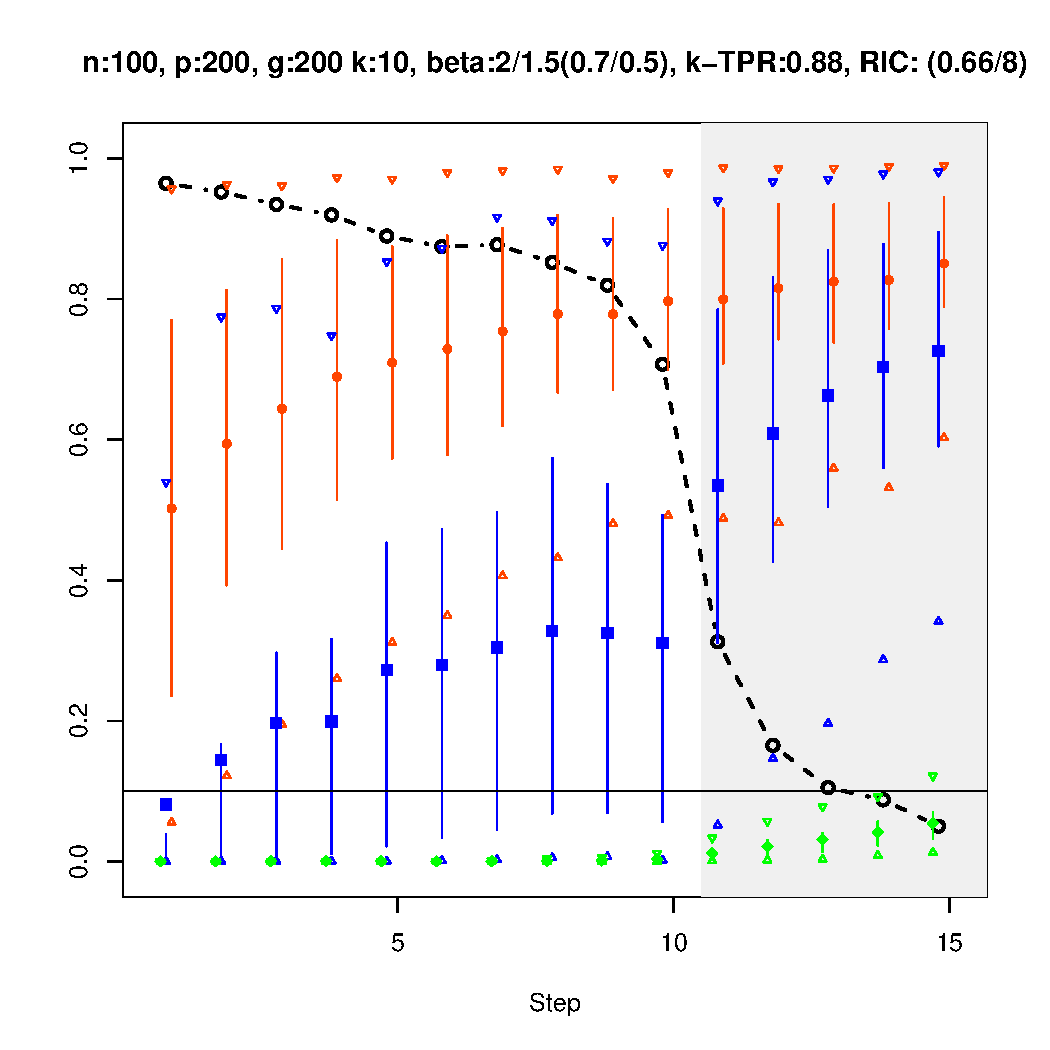
\includegraphics[width=0.5\textwidth]{../figs/default_gaussian_nsim400_n100_p200_g200_k10_lower1pt5_upper2_corr0pt2_noisecorr0pt1.pdf}}
\hspace{-15pt}
\subfigure[Gaussian with groups]{
\label{fig:gaussgroups}
\includegraphics[width=0.5\textwidth]{../figs/default_gaussian_nsim500_n100_p200_g35_sizes5-10_k5_lower2_upper3.pdf}}
\caption{\small \it The left panel shows results for Gaussian design
matrices with equicorrelation $\rho=0.2$ and equicorrelated noise with
correlation 0.1. The right panel shows results for an independent
Gaussian design with groups of sizes 5 and 10.}
\end{center}
\end{figure}

We show two types of plots, one containing the same information as in
Figure~\ref{fig:fwdstepsim}. The other plots each show a scenario with
a fixed sparsity level and contain the following information. The
horizontal axis is the step index for forward stepwise. The dashed
line shows the proportion of iterations where a truly nonzero variable
was added to the model at that step. Solid verticle lines are essentially
narrow boxplots, showing the middle 50\% of p-values calculated at that
step with circular points in these lines as the average and triangles
showing the 95\% and 5\% quantiles. Different color verticle lines
represent the following: red are calculated using our p-value on a null
model with no nonzero groups, blue are calculated on the non-null
model, and green calculated on the non-null model using the usual
$\chi^2$ significance test.

\begin{figure}[h]
\begin{center}
\subfigure[Real data categorical design]{
\label{fig:hivnrti}
\includegraphics[width=0.5\textwidth]{../figs/default_fixed_nsim100_n639_p354_g177_sizes2-2_k5_lower5_upper10.pdf}}
\hspace{-15pt}
\subfigure[Simulated categorical design]{
\label{fig:gausscat}
\includegraphics[width=0.5\textwidth]{../figs/default_categorical_nsim500_n100_p80_g40_sizes2-2_k5_lower2_upper4.pdf}}
\caption{\small \it The left panel shows results for a categorical design
taken from a real data set.
The right panel shows results for categorical matrices with all categories having 5 levels.}
\end{center}
\end{figure}

The performance of forward stepwise in these plots is characterized by how
close the dashed line is to a step function. If forward stepwise finds all
truly nonzero variables first this line will be close to 1 until the step
index reaches $k$ and then it will be close to 0. When this is the case,
our p-value tends to be small while forward stepwise is selecting truly
nonzero variables, uniform on the step where the dashed line goes to 0,
and then progressively larger afterward. A reasonable stopping rule based
on this behavior is to pick the model including all variables up to and
including the last one with a significant p-value. We call this the
\textit{last} stopping rule, and it selects the first $\hat k_\textit{last}$
variables in the forward stepwise path where, if
$p_j$ denotes our p-value calculated at the $j$-th step, then
\begin{equation}
  \label{eq:klast}
  \begin{aligned}
    \hat k_\textit{last} & = \max \{ j \leq steps : p_j < \alpha \}. \\
  \end{aligned}
\end{equation}
To test this stopping rule we compare it with several others which we now
describe. The \textit{oracle} stopping rule assumes knowledge of the
sparsity $k$ and always picks the first $k$ variables. The \textit{first}
rule stops immediately before the first variable to yield a p-value
larger than $\alpha$, and since this requires rejection of the global 
null in order to include the first variable
it controls the family-wise error rate. However it does not seem to have
good power.
The \textit{forward}
stopping rule is defined in \cite{sequential:fdr} and has the desirable
property that it controls the false discovery rate. Finally, \textit{RIC}
and \textit{BIC}
are the risk inflation criterion and Bayesian information criterion
described in Section~\ref{sec:fs:performance}. Tables~\ref{tab:easy} and
\ref{tab:hard} show simulation results with $\alpha = 0.1$.
To summarize these results, \textit{forward} is the only rule which
controls FDR, \textit{BIC} selects models that are far too large,
\textit{RIC} has low FDR and good power when the sparsity is low,
and \textit{last} is comparable to \textit{RIC},
with perhaps more power in the higher dimensional setting
(and a correspondingly larger FDR when the signal is also weak).



\begin{table}[ht]
\centering
\begin{tabular}{|r|r|lll|lll|lll|}
 \hline
   \multicolumn{2}{|c|}{p} & \multicolumn{3}{c|}{50}  & \multicolumn{3}{c|}{500} \\ 
  \hline \hline
    k & rule  &  R        & FDP        &  TPP          &   R      & FDP        & TPP \\ 
  \hline 
   & oracle  & 10(0)     & 0.06(0.08) & 0.94(0.08)  & 10(0) & 0.16(0.18) & 0.84(0.18) \\ 
   & first   & 1.5(1.5)  & 0(0.03)    & 0.14(0.14)  & 2.1(1.8) & 0.04(0.14) & 0.2(0.17) \\
10 & forward & 0.7(0.5)  & 0(0)       & 0.07(0.05)  & 0.8(0.4) & 0.01(0.11) & 0.08(0.04) \\
   & last    & 8.6(2)    & 0.03(0.06) & 0.84(0.19)  & 9.4(2.5) & 0.12(0.16) & 0.82(0.22) \\
   & RIC     & 9(2)      & 0.05(0.08) & 0.85(0.19)  & 6.2(3.5) & 0.09(0.15) & 0.57(0.33) \\
   & BIC     & 12(1.8)   & 0.17(0.11) & 0.98(0.05)  & 50(0) & 0.81(0.03) & 0.94(0.13) \\ 
  \hline
   & oracle  & 15(0)     & 0.07(0.07) & 0.93(0.07)  & 15(0) & 0.4(0.22) & 0.6(0.22) \\   
   & first   & 1.7(1.5)  & 0.01(0.09) & 0.11(0.1)   & 2.3(1.8) & 0.07(0.17) & 0.14(0.11) \\
15 & forward & 0.8(0.4)  & 0.01(0.1)  & 0.05(0.03)  & 0.8(0.4) & 0.04(0.2) & 0.05(0.03) \\
   & last    & 12.5(3.3) & 0.04(0.06) & 0.8(0.21)   & 11.4(4) & 0.29(0.22) & 0.53(0.25) \\
   & RIC     & 11.2(4.1) & 0.05(0.08) & 0.71(0.27)  & 3.6(2.8) & 0.11(0.2) & 0.21(0.17) \\
   & BIC     & 16.9(2.3) & 0.14(0.09) & 0.96(0.09)  & 50(0) & 0.78(0.07) & 0.73(0.23) \\ 

  \hline
\end{tabular}
\caption{Evaluation of model selection characteristics using several stopping rules.
  Here $n$ is fixed at 100, $p$ has 50 or 500 independent gaussian vectors,
  and the sparsity $k$ is set to 10 or 15.
  Nonzero coefficients have magnitudes in $[1.5\gamma, 2\gamma]$ for
  $\gamma = \sqrt{2\log (p)/n}$. The average over 400 simulations of the selected model
  size  (R), false discovery proportion  (FDP), and true positive proportion  (TPP)
  are shown with Monte Carlo standard errors in parentheses.}
\end{table}

 %    & first   & 1.3 (1.3)  & 0 (0.04)    & 0.26 (0.25)    & 1.8 (1.5) & 0.02 (0.11) & 0.36 (0.3) \\
 %    & forward & 0.6 (0.5)  & 0 (0)       & 0.13 (0.1)     & 0.8 (0.4) & 0.01 (0.1)  & 0.15 (0.09) \\
 %  5 & last    & 4.2 (1.3)  & 0.03 (0.08) & 0.82 (0.22)    & 4.7 (1.1) & 0.04 (0.11) & 0.88 (0.18) \\
 %    & RIC     & 4.7 (1)    & 0.06 (0.1)  & 0.89 (0.16)    & 5 (1.1)   & 0.08 (0.13) & 0.91 (0.18) \\
 %    & BIC     & 6.7 (1.5)  & 0.25 (0.16) & 0.97 (0.08)    & 50 (0)    & 0.9 (0.01)  & 0.98 (0.07) \\  
 %  \hline
 %    & first   & 1.4 (1.4)  & 0.01 (0.05) & 0.14 (0.14)    & 1.9 (1.5) & 0.03 (0.1)  & 0.18 (0.14) \\
 %    & forward & 0.7 (0.5)  & 0 (0.07)    & 0.07 (0.05)    & 0.8 (0.4) & 0.01 (0.1)  & 0.08 (0.04) \\
 % 10 & last    & 8 (2.4)    & 0.02 (0.06) & 0.78 (0.22)    & 8.3 (2.3) & 0.1 (0.15)  & 0.74 (0.23) \\
 %    & RIC     & 8.3 (2.4)  & 0.05 (0.08) & 0.79 (0.22)    & 5.5 (3)   & 0.09 (0.13) & 0.5 (0.29) \\ 
 %    & BIC     & 11.6 (1.8) & 0.16 (0.12) & 0.96 (0.08)    & 50 (0)    & 0.82 (0.03) & 0.92 (0.14) \\ 


\begin{table}[ht]
\centering
\begin{tabular}{|r|r|lll|lll|lll|}
 \hline
   \multicolumn{2}{|c|}{p} & \multicolumn{3}{c|}{50}  & \multicolumn{3}{c|}{500} \\ 
  \hline \hline
    k & rule  &  R        & FDP        &  TPP          &   R      & FDP        & TPP \\ 
  \hline
   & oracle  & 15(0)     & 0.18(0.09) & 0.82(0.09)  & 15(0) & 0.54(0.17) & 0.46(0.17) \\
   & first   & 1.1(1.1)  & 0(0.06)    & 0.07(0.07)  & 1.5(1.3) & 0.08(0.22) & 0.09(0.08) \\
15 & forward & 0.6(0.5)  & 0(0.05)    & 0.04(0.03)  & 0.7(0.4) & 0.05(0.21) & 0.05(0.03) \\
   & last    & 6.3(3.7)  & 0.03(0.07) & 0.4(0.23)   & 7.2(3.6) & 0.28(0.25) & 0.32(0.17) \\
   & RIC     & 6.5(3.1)  & 0.06(0.1)  & 0.41(0.2)   & 2.4(1.8) & 0.12(0.24) & 0.14(0.11) \\
   & BIC     & 14.2(2.9) & 0.16(0.1)  & 0.79(0.15)  & 50(0) & 0.84(0.05) & 0.54(0.18) \\
  \hline
   & oracle  & 20(0)     & 0.17(0.08) & 0.83(0.08)  & 20(0) & 0.65(0.12) & 0.35(0.12) \\
   & first   & 1.3(1.2)  & 0.02(0.11) & 0.06(0.06)  & 1.6(1.4) & 0.12(0.26) & 0.07(0.06) \\
20 & forward & 0.7(0.5)  & 0.02(0.13) & 0.03(0.02)  & 0.7(0.4) & 0.07(0.25) & 0.03(0.02) \\
   & last    & 7.7(4.3)  & 0.05(0.09) & 0.36(0.2)   & 8.8(4.2) & 0.41(0.23) & 0.24(0.11) \\
   & RIC     & 6.1(2.9)  & 0.05(0.11) & 0.29(0.14)  & 2(1.5) & 0.14(0.27) & 0.08(0.07) \\ 
   & BIC     & 17.2(3.9) & 0.14(0.09) & 0.74(0.16)  & 50(0) & 0.84(0.05) & 0.4(0.12) \\ 

  \hline
\end{tabular}
\caption{As in the previous table, but here the sparsity $k$ is set to 15 or 20
  and nonzero coefficients have magnitudes in $[1.1\gamma, 1.5\gamma]$ for
  $\gamma = \sqrt{2\log(p)/n}$. }
\end{table}

  %    & first   & 0.8 (0.9) & 0 (0.03)    & 0.08 (0.09)  & 1 (1) & 0.05 (0.19) & 0.09 (0.09) \\  
  %    & forward & 0.6 (0.5) & 0 (0)       & 0.06 (0.05)  & 0.6 (0.5) & 0.04 (0.21) & 0.06 (0.05) \\
  % 10 & last    & 3.4 (2.6) & 0.03 (0.09) & 0.32 (0.24)  & 4 (2.6) & 0.19 (0.25) & 0.29 (0.19) \\
  %    & RIC     & 4.5 (2.1) & 0.06 (0.12) & 0.42 (0.21)  & 2.5 (1.8) & 0.15 (0.27) & 0.21 (0.15) \\
  %    & BIC     & 9.3 (2.3) & 0.2 (0.15)  & 0.74 (0.18)  & 50 (0) & 0.87 (0.04) & 0.64 (0.21) \\ 
  % \hline
  %    & first   & 1 (1)     & 0 (0.05)    & 0.06 (0.06)  & 1.2 (1.1) & 0.09 (0.25) & 0.07 (0.07) \\
  %    & forward & 0.6 (0.5) & 0 (0)       & 0.04 (0.03)  & 0.7 (0.5) & 0.08 (0.26) & 0.04 (0.03) \\
  % 15 & last    & 4.7 (3.1) & 0.04 (0.09) & 0.3 (0.19)   & 5.9 (3.3) & 0.26 (0.26) & 0.27 (0.16) \\
  %    & RIC     & 5 (2.7)   & 0.05 (0.11) & 0.32 (0.17)  & 2.2 (1.8) & 0.12 (0.24) & 0.13 (0.11) \\
  %    & BIC     & 12.8 (3)  & 0.17 (0.11) & 0.7 (0.17)   & 60 (0) & 0.86 (0.04) & 0.55 (0.17) \\ 


% & \multicolumn{3}{c|}{200}
% &  R         & FDP        & TPP       
                                      
% & 1.5  (1.4)   & 0  (0.04)    & 0.3  (0.28) 
% & 0.7  (0.4)   & 0  (0)       & 0.15  (0.09)
% & 4.6  (1.2)   & 0.05  (0.11) & 0.87  (0.19)
% & 4.9  (1.1)   & 0.07  (0.12) & 0.89  (0.18)
% & 35  (16.3)   & 0.8  (0.14)  & 0.98  (0.07)
                                      
% & 1.8  (1.5)   & 0.01  (0.07) & 0.18  (0.15)
% & 0.8  (0.4)   & 0  (0)       & 0.08  (0.04)
% & 8.1  (2.7)   & 0.08  (0.12) & 0.75  (0.25)
% & 6.6  (3.1)   & 0.07  (0.11) & 0.61  (0.3) 
% & 42.9  (12.3) & 0.74  (0.13) & 0.96  (0.08)


\section{Applications}
\label{sec:applications}
We now turn to applying forward stepwise and examining the behavior of
our test statistic in several unique settings, including a real data
example.

\subsection{Nonlinear regression with splines}

\begin{figure}
\begin{center}
\subfigure[Power of forward stepwise with splines]{
\label{fig:spline:fwd}
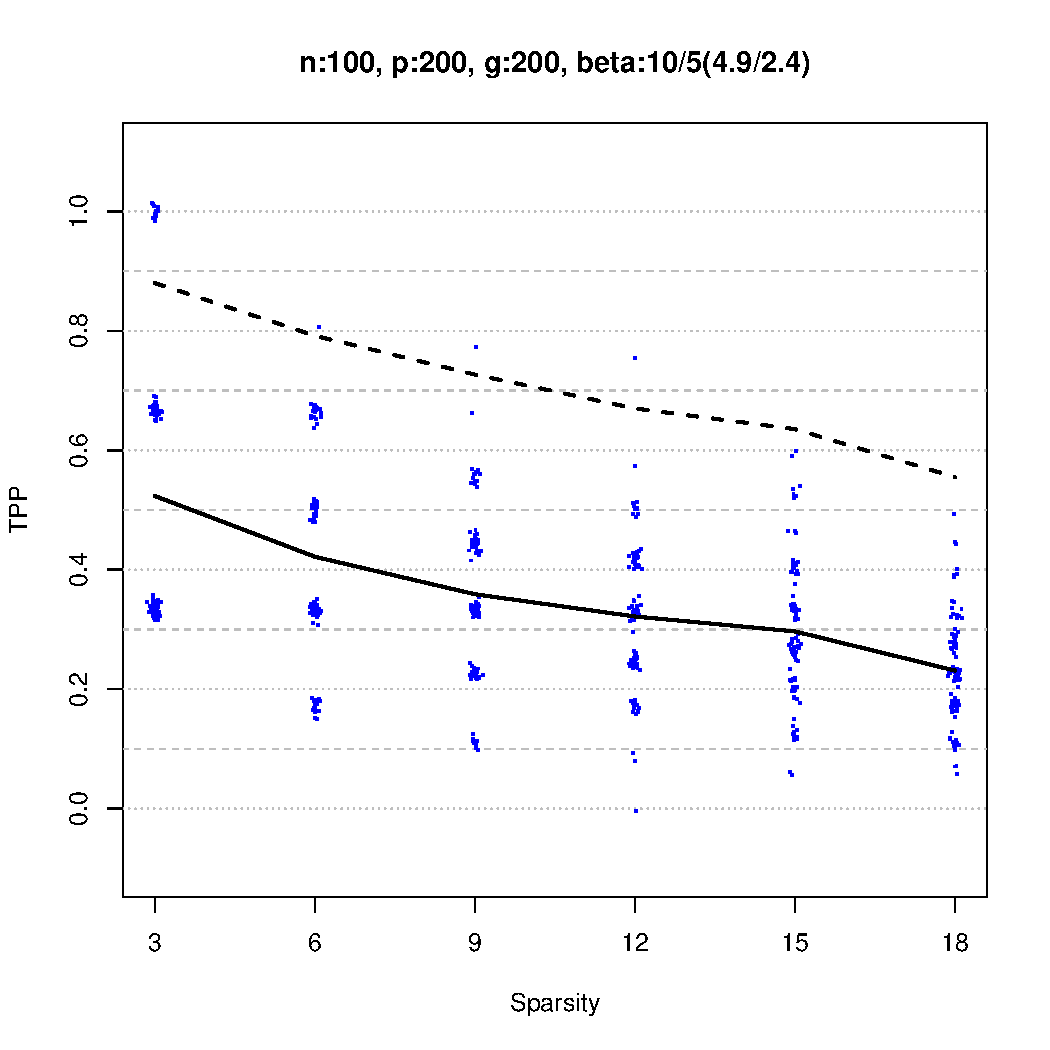
\includegraphics[width=0.5\textwidth]{../figs/tpr_gamsel_uniform_nsim100_n100_p200_g200_k18_k01_lower5_upper10.pdf}}
\hspace{-15pt}
\subfigure[P-value with spline groups]{
\label{fig:spline:pval}
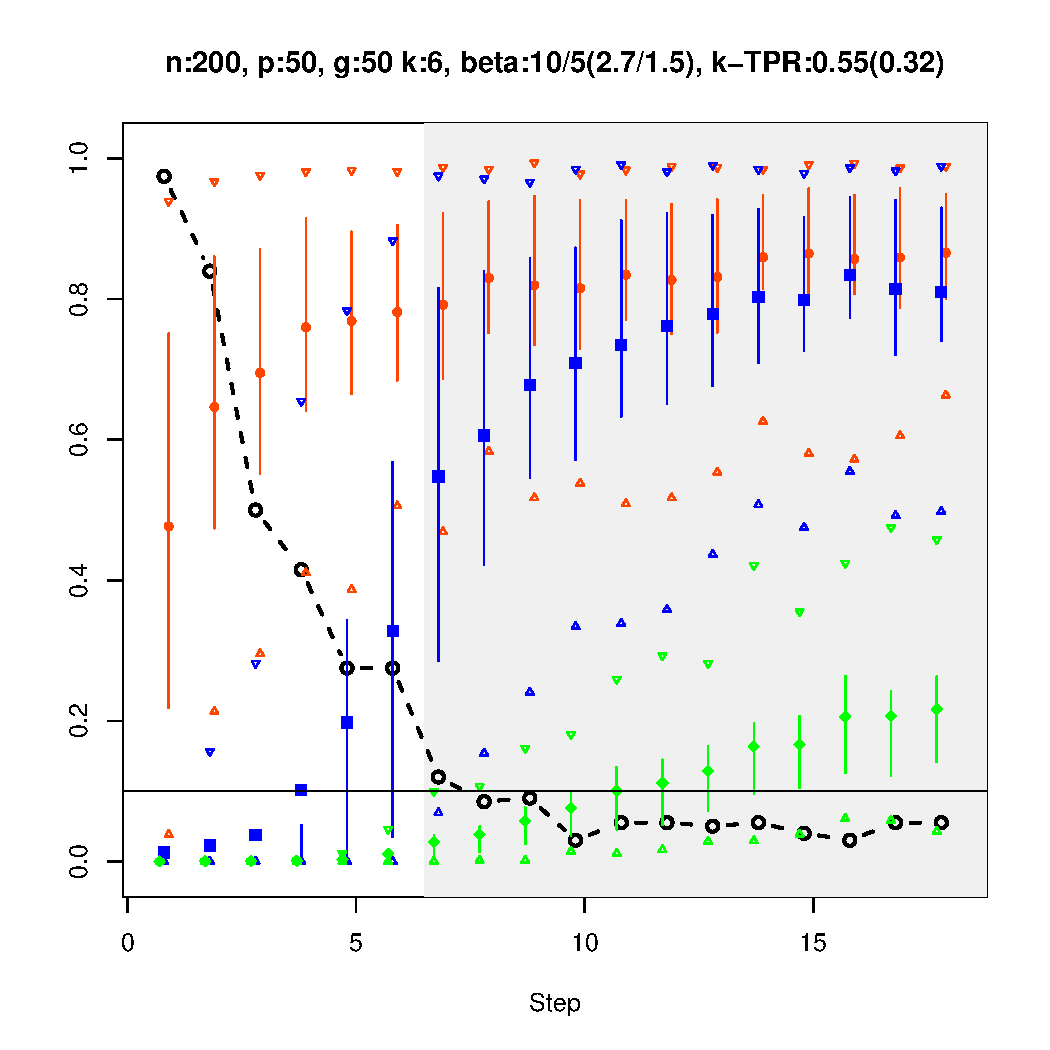
\includegraphics[width=0.5\textwidth]{../figs/gamsel_uniform_nsim200_n200_p50_g50_k6_k02_lower5_upper10.pdf}}
\caption{\small \it The left panel shows the power of forward stepwise
in this setting for various sparsity levels, with the dashed line
showing a liberal definition of power that allows mistakes when
choosing between a non-zero spline group and its corresponding linear
term.
The right panel shows our p-value marginally
over each step, with red indicating the global null case, blue
indicating a signal with $k=6$ nonzero groups, and green showing
the nominal $\chi^2$ p-values also computed on the non-null case.}
\label{fig:spline}
\end{center}
\end{figure}

First we consider a simple extension of the usual linear regression setting. Given a design matrix $X$, we can augment this by adding additional columns given by nonlinear functions of the original covariates. Specifically, we compute spline basis vectors for each covariate and create a group given by this spline basis. Denote this new design matrix
\begin{equation}
\label{eq:splinemat}
  \begin{aligned}
    \tilde X &=  \begin{pmatrix} X_1 & \cdots & X_G & X^+_1 & \cdots & X^+_G  \end{pmatrix}\\
    &= \begin{pmatrix} X & X^+ \end{pmatrix}
  \end{aligned}
\end{equation}
with $\tilde G = 2G$ groups. For simplicity we assume the original groups are all size 1, and use the B-spline basis. In our simulations we generate original covariates uniformly in the interval [-1,1] and use cubic splines with boundary knots
\begin{equation}
  \begin{aligned}
    X_i &\sim \text{Unif}[-1,1], \quad
    X_i^+ = \text{CubicSplineBasis}(X_i)
  \end{aligned}
\end{equation}
Nonzero coefficients are split between original covariates and spline groups. Simulation results are shown in Figure~\ref{fig:spline}. Note that the varying group sizes present some difficulty to forward stepwise, which tends to first try linear approximations to nonzero spline groups before adding the true spline group. In Figure~\ref{fig:spline}(b) the average proportion of truly nonzero spline groups included in the first $k$ steps appears in parentheses next to the $k$-TPP (top right).


\subsection{Glinternet for hierarchical interactions}
\label{sec:glint}
In regression settings with many variables, choosing among models with pairwise interactions can drastically increase model complexity. \cite{glint} propose a method called \textsc{glinternet} to reduce the statistical complexity of this problem. The method imposes a strong hierarchical constraint on interactions (similar to that in \cite{bien:hierarchical}) where an interaction term can only be included if both its main effects are also included. They accomplish this by creating a design matrix with both main effects alone and also with groups including main effects with their first order interactions. Then they fit a group LASSO model with the expanded design matrix. Because interaction terms only appear in groups along with their respective main effects, the hierarchy condition holds for the fitted model. We now consider a related procedure as an example problem, but first modify their method to simplify some parts. Let the expanded design matrix be given by
\begin{equation}
\label{eq:glintmat}
\tilde X = \begin{pmatrix} X_1 & \cdots & X_G & X_{1:2} & \cdots & X_{1:G} & X_{2:3} & \cdots & X_{(G-1):G}  \end{pmatrix}
\end{equation}
where $X_{g:h}$ is the submatrix encoding the interaction between $X_g$
and $X_h$. For example, if both of these are categorical variables,
then $X_{g:h}$ consists of all
$p_gp_h$  column multiples between columns in group $g$ and columns
in group $h$. For example, if
\[
X_g = \begin{pmatrix} X_{g1} & X_{g2} \end{pmatrix}, \quad
X_h = \begin{pmatrix} X_{h1} & X_{h2} \end{pmatrix}
\]
are two categorical variables each with two levels, then
\[
X_{g:h} = \begin{pmatrix} X_{g1} * X_{h1} & X_{g1} * X_{h2} & X_{g1} * X_{h1} & X_{g2} * X_{h2} \end{pmatrix}
\]
where * denotes the pointwise product (Hadamard product) of vectors
(the $i$th entry of $X_{g1} * X_{h1}$ is the $i$th entry of $X_{g1}$ times
the $i$th entry of $X_{h1}$). For more details see \cite{glint}.
Note that this expanded matrix has
$\tilde G = G + \binom{G}{2} = O(G^2)$ groups. We refer to the first
$G$ of these as main effect groups and the remaining
as interaction groups. Finally, instead of fitting a
model by group LASSO, we use forward stepwise on the expanded design
matrix. The overlapping groups still guarantee that our fitted model
satisfies the strong hierarchy condition. 

%However, we must first modify our implementation of forward stepwise to prevent the possibility of including main effect groups after the main effects are already included in the model as part of an interaction group. To do this we compute the residual using the whole model in each step, rather than by subtracting the effect of the current group being included. For a set of group indices $A \subseteq \{ 1, \ldots G \}$ we write $X_A$ for the submatrix of the design matrix containing all the groups in $A$.
% \begin{algorithm}
% \DontPrintSemicolon
% \caption{\small \it Modification to compute residual from full model}
% \BlankLine
% \CommentSty{\# Everything the same as before, additionally:}\;
% %  $P_A \gets I - X_AX_A^\dagger$\;
% %  $r_s \gets P_A r_{s-1}$\;
% \If{$g^*$ is an interaction group}{
%   $g_1, g_2 \gets$ main effects groups of $g^*$\;
%   A^c \gets A^c \slash \{ g_1, g_2 \}\;
% }%\;
% %$r_s \gets y - \text{lsfit}(X_A, y)$\;
% \BlankLine
% \label{algo:fs:full}
% \end{algorithm}
% \begin{algorithm}
% \DontPrintSemicolon
% \KwData{An $n$ vector $y$ and $n \times p$ matrix $X$ of $G$ groups of variables}
% \KwResult{Active set $A$ of variable groups included in the model}
% \SetKwFunction{lsfitResidual}{lsfitResidual}
% \caption{\small \it Forward stepwise for glinternet}
% \BlankLine
% Compute design matrix~(\ref{eq:glintmat}) and expanded grouping $\tilde G$\;
% $A \gets \emptyset$\;
% $A^c \gets \{ 1, \ldots, G \}$\;
% $r_0 \gets y$\;
% \For{$s \gets 1$ \KwTo $steps$}{
%   $g^* \gets \argmax_{g \in A^c} \{ \norm{X_g^T r_{s-1}}_2 / w_g \}$\;
%   $P \gets I - X_{g^*}X_{g^*}^\dagger$\;
%   $A \gets A \cup \{ g^* \}$\;
%   $A^c \gets A^c \backslash \{ g^* \}$\;
%   \For{$g \in A^c$}{
%     $X_g \gets P X_g$\;
%   }
%   $r_s \gets P r_{s-1}$\;
% }
% \KwRet{$A$}
% \label{algo:fsgl}
% \end{algorithm}

To demonstrate this method by simulation, we constructed signals which have
the first $k/3$ main effects nonzero but with no interactions, and the
remaining $2k/3$ nonzero main effects are matched to each other to form
interactions.
%This way each nonzero main effect with any nonzero interactions has
%exactly one nonzero interaction. 
We also inflate each nonzero interaction
coefficient to be larger than the corresponding main
effect coefficients. This special case is favorable for our algorithm,
but our purpose here is merely to demonstrate the flexibility of the
hypothesis test and not to propose an optimal procedure for models with
interactions.

Results are shown in Figure~\ref{fig:glint}. The left
panel shows average power of forward stepwise. Power is calculated
using the group structure we impose, and not in terms of the original
main effects and interactions. However, the dashed line shows a more
forgiving definition of power where we are rewarded for discovering part
of a nonzero group, i.e. for discovering only one main effect from a
true interaction group. The proportion of nonzero interaction groups
that were discovered in the first $k$-steps is shown in parentheses
after the $k$-TPP (top right).

\begin{figure}
\begin{center}
\subfigure[Power of forward stepwise with interactions]{
\label{fig:glint:fwd}
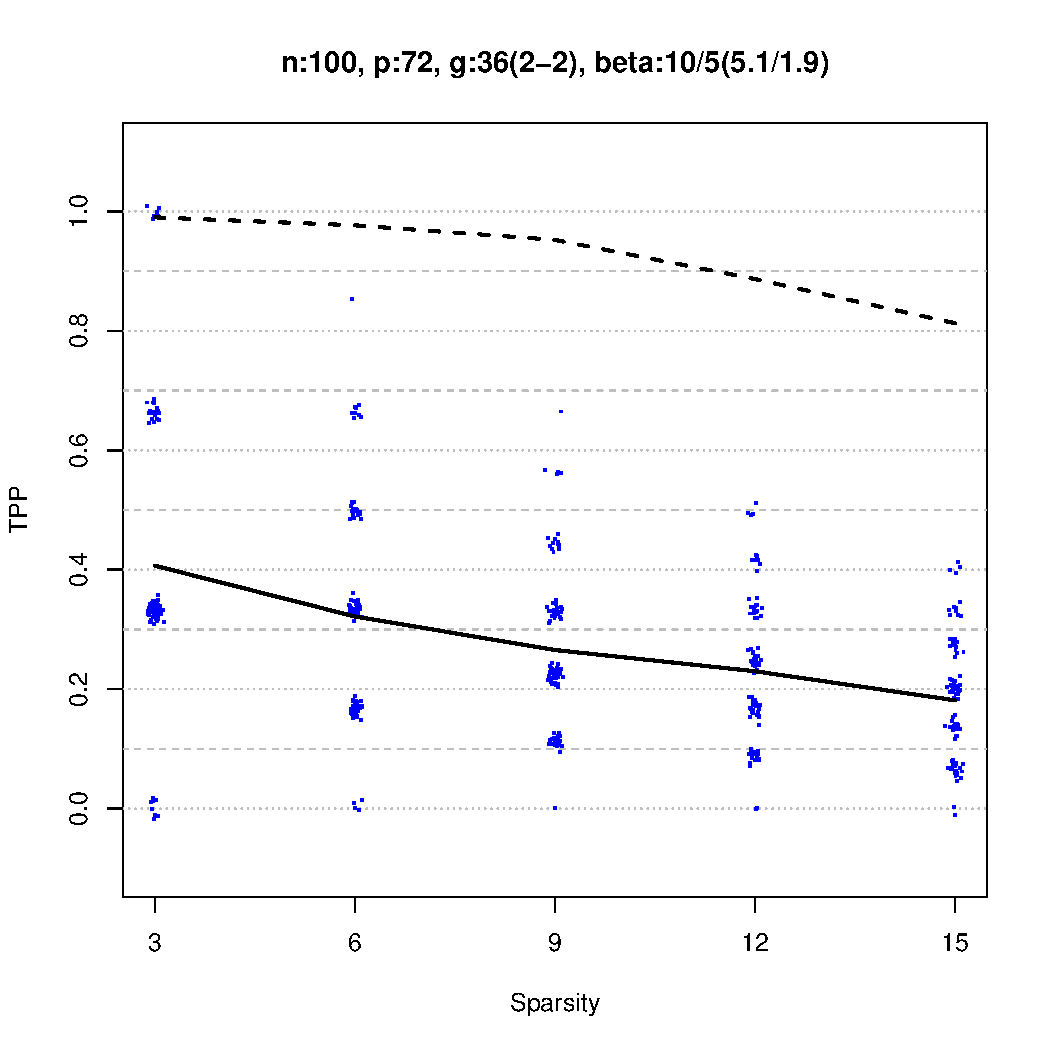
\includegraphics[width=0.5\textwidth]{../figs/tpr_glint_categorical_nsim100_n100_p72_g36_sizes2-2_k15_k01_lower5_upper10.pdf}}
\hspace{-15pt}
\subfigure[P-value with \textsc{glinternet}]{
\label{fig:glint:pval}
\includegraphics[width=0.5\textwidth]{../figs/glint_gaussian_nsim100_n100_p30_g30_k6_k02_lower4_upper8.pdf}}
\caption{\small \it The left panel shows the power of forward stepwise
on the \textsc{glinternet} problem
for various sparsity levels. The dashed line shows a more forgiving
definition of power described in the section.
The right panel shows our p-value marginally
over each step, with red indicating the global null case, blue
indicating a signal with $k=6$ nonzero groups, and green showing
the nominal $\chi^2$ p-values.}
\label{fig:glint}
\end{center}
\end{figure}



\subsection{HIVdb data example}
\label{sec:hiv}

\cite{HIV} use genomic information to predict efficacy of antiretroviral
drugs in treating HIV. Quantitative measurements of drug
response/resistance were regressed on categorical covariates encoding
the presence and type of certain genetic mutations. We attempt a similar
analysis using forward stepwise, and report our P-value at each step.
Categorical covariates are encoded as groups of binary variables using
the full encoding, and weights are set to the square-root of the
number of levels for that covariate. We perform forward stepwise once
for each drug response, restricting to the subset of the data with
no missing values.

\begin{figure}
\begin{center}
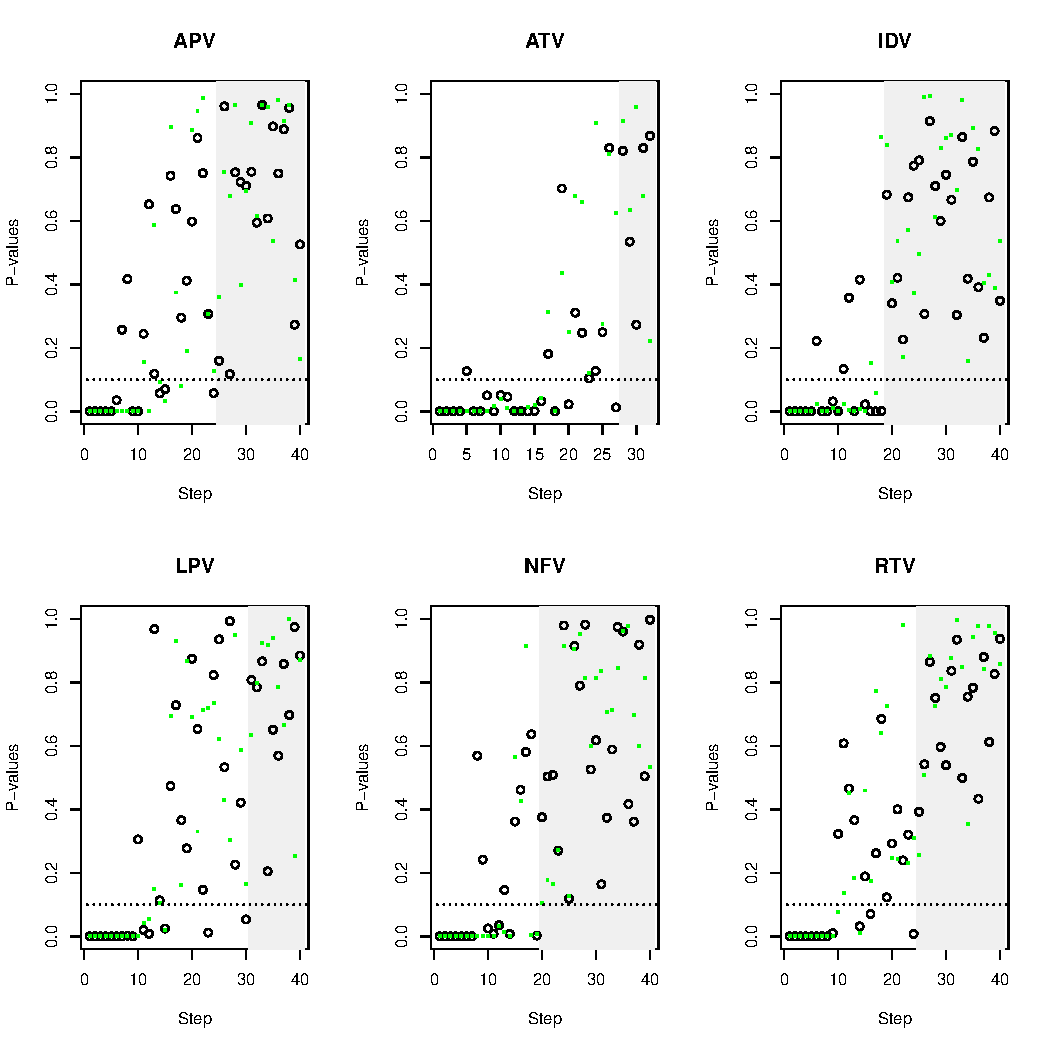
\includegraphics[width=0.9\textwidth]{../figs/HIV_PI.pdf}
\caption{\small \it Forward stepwise results from PI dataset}
\label{fig:HIVPI}
\end{center}
\end{figure}

\begin{figure}
\begin{center}
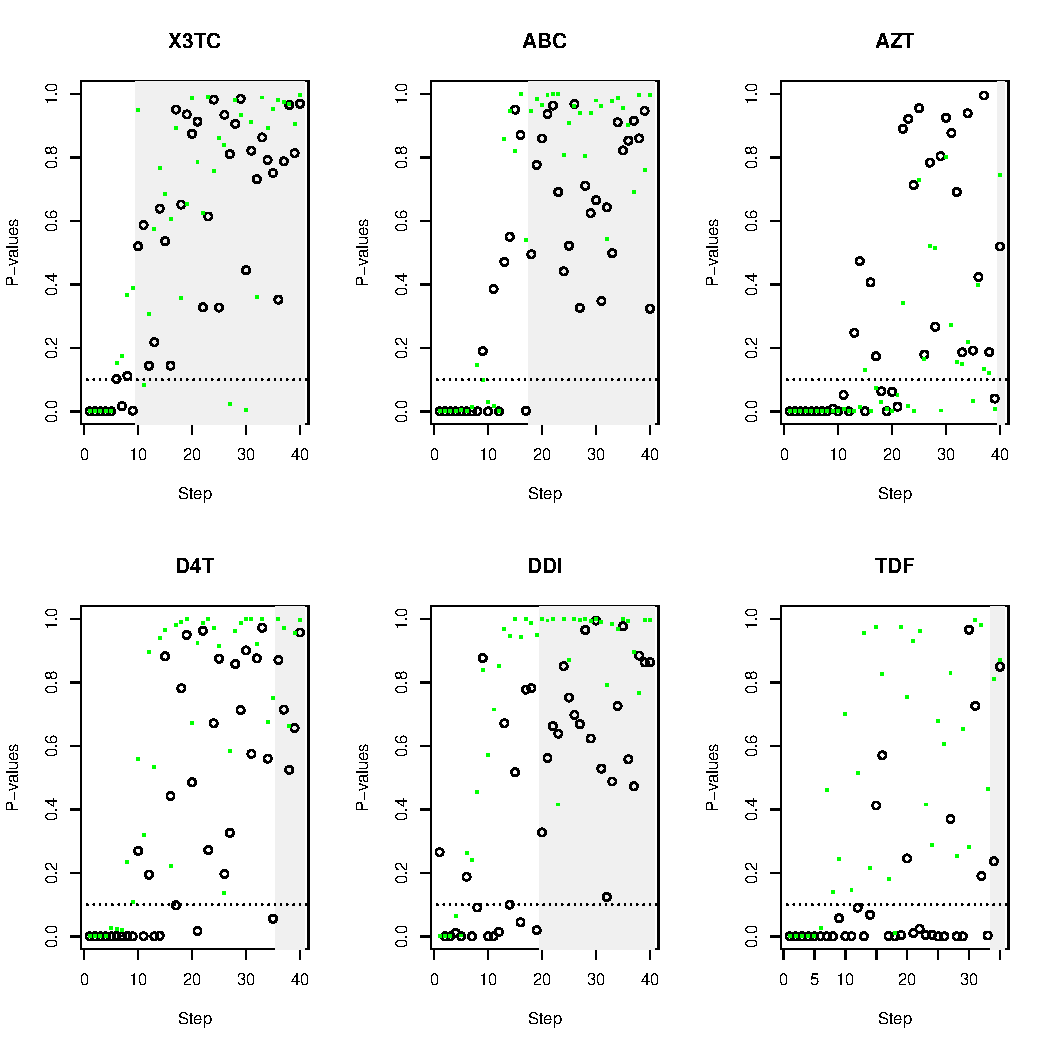
\includegraphics[width=0.9\textwidth]{../figs/HIV_NRTI.pdf}
\caption{\small \it Forward stepwise results from NRTI dataset}
\label{fig:HIVNRTI}
\end{center}
\end{figure}

Results from two data sets are displayed in Figure~\ref{fig:HIVPI} and
Figure~\ref{fig:HIVNRTI}. The PI data contains protease inhibitor
resistance mutations, and the NRTI data contains nucleoside RT inhibitor
resistance mutations.
Each panel shows results for a different drug,
with p-values plotted by step in forward stepwise. 
The \textit{last} stopping rule is applied and the region of the plot
corresponding to the chosen model is unshaded, with the remainder shaded.
The chosen variables are shown in Tables~\ref{tab:hivPI} and
\ref{tab:hivNRTI}.

%\begin{figure}
%\begin{center}
% latex table generated in R 3.0.2 by xtable 1.7-1 package
% Wed May 14 17:30:50 2014
\begin{table}[ht]
\centering
\begin{tabular}{rllll}
  \hline
 & Drug & n & G & Selected variables \\ 
  \hline
1 & APV & 768 & 82 & P90 P46 P54 P84 P88 P32 P50 P76 P33 P10 P15 P82 P93 P24 P47 P64 P58 P11 P43 P35 P77 P63 P13 P48 \\ 
  2 & ATV & 329 & 71 & P90 P54 P84 P50 P30 P32 P24 P76 P62 P46 P35 P88 P82 P73 P58 P43 P77 P48 P64 P36 P13 P14 P74 P71 P11 P57 P20 \\ 
  3 & IDV & 827 & 82 & P90 P46 P54 P84 P82 P62 P88 P73 P35 P50 P71 P24 P76 P32 P48 P10 P20 P63 \\ 
  4 & LPV & 517 & 76 & P90 P54 P46 P84 P36 P82 P76 P47 P50 P10 P73 P33 P53 P24 P48 P62 P93 P11 P71 P60 P14 P19 P20 P41 P70 P13 P16 P37 P88 P30 \\ 
  5 & NFV & 844 & 82 & P90 P46 P30 P54 P84 P36 P88 P73 P24 P82 P50 P71 P10 P74 P77 P35 P63 P20 P48 \\ 
  6 & RTV & 795 & 82 & P90 P54 P46 P84 P82 P36 P24 P50 P32 P73 P13 P15 P88 P30 P35 P33 P93 P71 P10 P58 P53 P63 P48 P20 \\ 
  7 & SQV & 826 & 82 & P90 P84 P54 P30 P48 P36 P24 P53 P88 P73 P15 P82 P10 P71 P76 P58 P93 P74 P50 P63 P62 P20 P14 P41 P46 P32 P57 P70 P67 P43 P13 P16 \\ 
   \hline
\end{tabular}
\caption{Variables chosen using \textit{last} stopping rule in forward stepwise} 
\end{table}


%\label{tab:HIVPI}
%\end{center}
%\end{figure}

%\begin{figure}
%\begin{center}
% latex table generated in R 3.0.2 by xtable 1.7-1 package
% Mon May  5 22:18:44 2014
\begin{table}[ht]
\centering
\begin{tabular}{rllll}
  \hline
Drug & n & G & $\hat k$ & Selected variables \\ 
  \hline
X3TC & 633 & 176 & 9 & P184 P41 P65 P67 P151 P210 P181 P83 P215 \\ 
ABC & 628 & 176 & 17 & P184 P41 P151 P67 P210 P65 P74 P83 P218 P215 P115 P69
\ldots  \\% P60 P43 P202 P200 P219 \\ 
AZT & 630 & 176 & 39 & P41 P67 P184 P151 P210 P70 P74 P215 P181 P77
P103 P69 \ldots \\ % P203 P218 P135 P100 P196 P35 P43 P219 P208 P98 P118 P221 P83 P169 P142 P178 P227 P162 P60 P65 P121 P21 P111 P44 P68 P108 P94 \\ 
D4T & 630 & 176 & 35 &P41 P151 P67 P210 P184 P69 P65 P218 P215 P118 P75 P83
\ldots \\ % P219 P181 P214 P77 P203 P20 P122 P40 P44 P70 P103 P221 P90 P119 P116 P74 P6 P177 P35 P100 P200 P94 P85 \\ 
DDI & 632 & 176 & 19 & P184 P151 P41 P74 P65 P67 P210 P218 P83 P75 P69
P118
\ldots \\ % P214 P215 P179 P106 P123 P70 P219 \\ 
TDF & 353 & 153 & 33 &P41 P184 P70 P210 P65 P74 P181 P62 P215 P68 P67 P98
\ldots \\ %P35 P151 P196 P202 P75 P118 P135 P218 P203 P122 P6 P115 P69 P103 P60 P121 P21 P77 P39 P142 P100 \\ 
   \hline
\end{tabular}
\caption{Variables chosen using \textit{last} stopping rule in forward
  stepwise on HIVdb NRTI dataset} 
\label{tab:hivNRTI}
\end{table}


%\label{tab:HIVNRTI}
%\end{center}
%\end{figure}

We can also use the \textsc{Glinternet} procedure described in Section~\ref{sec:glint} to fit a model with pairwise interactions. Results from this are shown in Figures~\ref{fig:HIVPI:glint} and \ref{fig:HIVNRTI:glint} and Tables~\ref{tab:glintPI} and \ref{tab:glintNRTI}.

\begin{figure}
\begin{center}
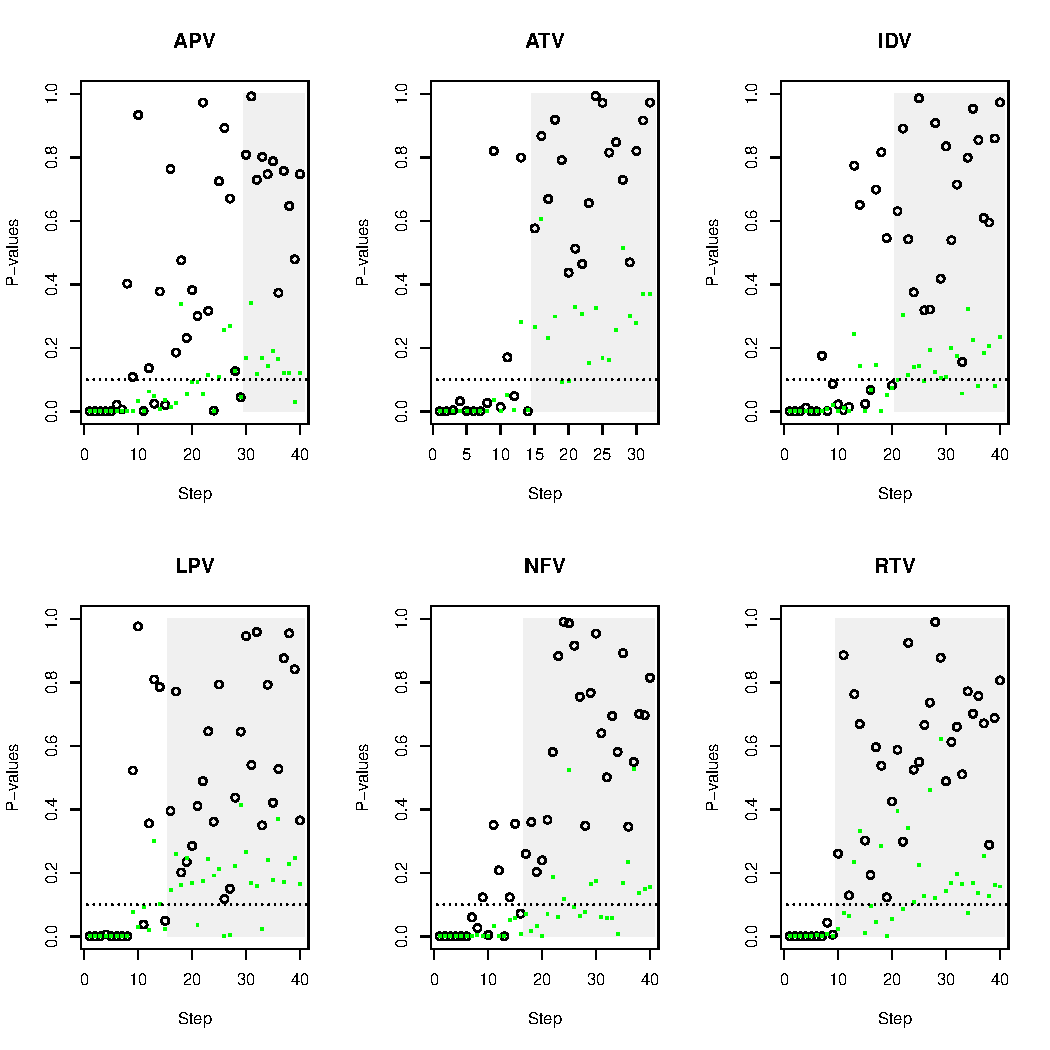
\includegraphics[width=0.9\textwidth]{../figs/HIV_PI_glint.pdf}
\caption{\small \it \textsc{Glinternet} results from PI dataset}
\label{fig:HIVPI:glint}
\end{center}
\end{figure}

\begin{figure}
\begin{center}
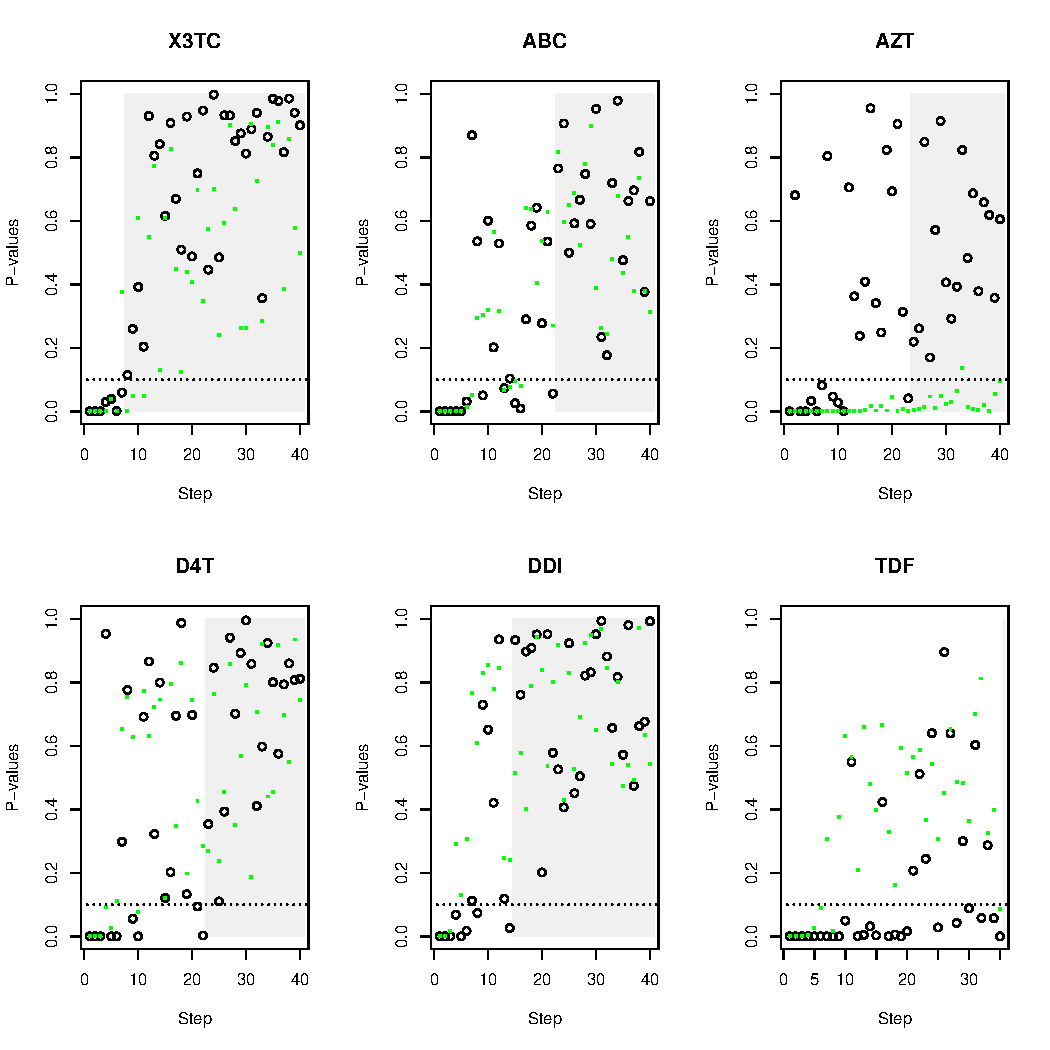
\includegraphics[width=0.9\textwidth]{../figs/HIV_NRTI_glint.pdf}
\caption{\small \it \textsc{Glinternet} results from NRTI dataset}
\label{fig:HIVNRTI:glint}
\end{center}
\end{figure}


% latex table generated in R 3.0.2 by xtable 1.7-1 package
% Tue May  6 00:00:24 2014
\begin{table}[ht]
\centering
\begin{tabular}{rllll}
  \hline
Drug & n & G & $\hat k$ & Selected variables \\ 
  \hline
APV & 768 & 3403 & 29 &P8*P10 P7*P46 P54*P84 P76*P90 P30*P88 P33*P50
P64*P93
\ldots \\% P32*P48 P47*P71 P13*P89 P88*P90 P37*P85 P15*P62 P82*P84 P41*P66 P11*P60 P37*P46 P57*P63 P62*P90 P10*P93 P19*P93 P84*P90 P19*P36 P36*P50 P82*P93 P20*P62 P35*P62 P55*P72 P72*P82 \\ 
ATV & 329 & 2556 & &P10*P76 P8*P71 P20*P46 P33*P48 P50*P84 P79*P90 P30*P54 P32*P88 P62*P82 P73*P74 P35*P53 P24*P43 P64*P77 P58*P67 \\ 
IDV & 827 & 3403 & &P10*P26 P46*P54 P48*P90 P20*P24 P82*P84 P71*P88 P15*P73 P41*P63 P62*P89 P30*P50 P71*P77 P84*P90 P36*P93 P36*P37 P67*P76 P43*P92 P12*P79 P48*P62 P20*P90 P62*P71 \\ 
LPV & 517 & 2926 & &P54 P46*P48 P10*P75 P20*P84 P82*P84 P33*P50 P76*P90 P47*P62 P64*P77 P53*P88 P37*P85 P24*P67 P19*P93 P36*P90 P36*P93 \\ 
NFV & 844 & 3403 & &P10*P30 P46*P90 P54*P88 P20*P84 P82*P84 P48*P73 P63*P76 P71*P77 P24*P74 P46*P82 P36*P69 P84*P90 P37*P50 P13*P33 P35*P46 P12*P79 \\ 
RTV & 795 & 3403 & &P82*P84 P24*P90 P39*P54 P36*P46 P10*P88 P63*P93 P15*P48 P46*P71 P33*P47 \\ 
SQV & 826 & 3403 & &P10*P76 P84*P90 P54*P88 P36*P48 P73*P74 P71*P93 P24*P53 P36*P90 P33*P82 P15*P20 P12*P64 P88*P90 P82*P90 \\ 
   \hline
\end{tabular}
\caption{Variables chosen using \textit{last} stopping rule in
  \textsc{Glinternet}} 
\label{tab:glintPI}
\end{table}



% latex table generated in R 3.0.2 by xtable 1.7-1 package
% Tue May  6 13:43:26 2014
\begin{table}[ht]
\centering
\begin{tabular}{rllll}
  \hline
  Drug & n & G & $\hat k$& Selected variables \\ 
  \hline
X3TC & 633 & 15576 & 7& P157*P184 P65*P215 P184*P215 P151*P210 P67*P75 \ldots \\ %P75*P184 P69*P123 \\ 
ABC & 628 & 15576 & 22&P54*P184 P151*P215 P65*P210 P69*P74 P184*P215 \ldots \\
% P41*P74 P115*P219 P83*P200 P174*P181 P106*P177 P35*P202 P190*P218 P184*P210 P35*P69 P69*P184 P41*P69 P75*P98 P39*P228 P103*P210 P196*P210 P41*P211 P62*P162 \\ 
AZT & 630 & 15576 & 23&P77*P215 P67*P151 P151*P184 P70*P210 P135*P214 \ldots \\
% P41*P74 P35*P202 P103*P203 P39*P69 P181*P196 P67*P184 P142*P228 P103*P210 P178*P190 P162*P169 P83*P219 P43*P98 P68*P207 P62*P218 P200*P202 P39*P135 P69*P122 P20*P228 \\ 
D4T & 630 & 15576 & 22&P151*P215 P65*P210 P67*P69 P104*P184 P75*P218 \ldots \\
% P41*P75 P122*P197 P123*P211 P35*P202 P35*P69 P20*P83 P70*P181 P60*P118 P62*P103 P69*P215 P74*P214 P103*P210 P162*P228 P69*P181 P219*P221 P43*P219 P215*P219 \\ 
DDI & 632 & 15576 & 14&P41*P151 P65*P184 P69*P74 P62*P219 P75*P210 \ldots \\
% P184*P215 P83*P179 P106*P135 P35*P70 P123*P138 P43*P218 P173*P181 P69*P70 P35*P69 \\ 
TDF & 353 & 11781 & 35&P41*P65 P184*P224 P32*P70 P68*P210 P174*P181 \ldots \\
% P74*P215 P35*P202 P62*P75 P103*P219 P135*P190 P11*P179 P190*P203 P162*P196 P122*P215 P44*P98 P20*P173 P69*P181 P103*P210 P39*P123 P200*P202 P67*P184 P123*P211 P103*P118 P67*P177 P103*P135 P67*P178 P21*P169 P69*P228 P106*P121 P122*P123 P60*P108 P83*P142 P196*P219 P35*P122 P75*P219 \\ 
   \hline
\end{tabular}
\caption{\em Variables chosen using \textit{last} stopping rule in
  \textsc{Glinternet} on HIVdb NRTI dataset} 
\label{tab:glintNRTI}
\end{table}



\section{Discussion}
\label{sec:discuss}

Under the global null hypothesis $\beta = 0$, we have a test statistic
which we can use against the alternative of including the ``best''
predictor (the one chosen by forward stepwise).
This test statistic has an exact, finite sample distribution.
If we choose to include the variable, we are no longer in the global null
setting. However, by orthogonalizing both the response and the remaining
predictors with respect to the included variable, it is reasonable to
iterate the global null test. While not fully theoretically justified,
this method seems to work well in all our simulations. By this we mean that
the p-value tends to be small on the step when including the last truly
nonzero predictor, uniform on the following step, and subsequently
stochastically larger than uniform. This is in contrast to p-values
calculated from traditional variable-inclusion tests like the $\chi^2$
test, which tend to be smaller than uniform long after the last truly
nonzero predictor has been included.

When adding the next variable in forward stepwise, our hypothesis test
roughly depends on the improvement gained by this variable compared to
the next best variable. Thus, the p-value is small when there is a large
gap between the variable to be included and all the remaining variables.
If multiple predictors have truly nonzero coefficients that are close
in magnitude, the p-value may be large until forward stepwise reaches
the last one. This motivated us to consider the \textit{last} stopping
rule for model selection \eqref{eq:klast}. In simulations we
found this stopping rule to have good performance in terms of power
(true positive rate), comparable to that of RIC \citep{RIC}.
But it does not control the false discovery rate
unless the truly nonzero coefficients are large enough to guarantee
forward stepwise picks the corresponding variables before picking too
many noise variables.

The present work calculates p-values at each step ignoring the constraints
imposed by previous steps. Future work adjusting for all previous steps
is in progress, and may be able to give exact p-values at a step chosen
stochastically by procedures like BIC and RIC. The authors hope to
eventually release an R package implementing these methods.


\newpage

\bibliographystyle{ims}
%\bibliographystyle{acmtrans-ims}
\bibliography{paper}

\newpage

\appendix
\section{Linear fractional subproblem}
\label{app:closedform}

This appendix describes the \textsc{LinearFractional} optimization
subproblem and its solution.
The problem was named as it originated in the form
\[
\maximize_{h \neq g, \norm{u_h}_2 = 1}
\frac{u_h^TX_h^Ty - u_h^TX_h^T\tilde X_g \tilde X_g^Ty}
{1 - u_g^T \tilde X_g^TX_hu_h}
\]
The solution we describe next is to a slightly different problem which
also incorporates the information that $g$ maximizes $\norm{X_g^Ty}_2/w_g$.
Although the logic seems a bit complicated, it mainly involves ruling out
several cases as infeasible. The infeasibilities are precisely those given
by the characterization of the global maximizer in \cite{tests:adaptive}.
After ruling out degenerate cases, we obtain the following solution
by transforming to trigonometric coordinates and using calculus.

\begin{algorithm}
 \caption{The \textsc{LinearFractional} subproblem}
 \label{algo:linfrac}
 \begin{algorithmic}
   \REQUIRE The $p$-vectors $a, b$ in Algorithm~\ref{algo:pval}, weights, inactive set $A^c$, a small tolerance number
(we take $1e^{-10}$)
   \ENSURE Solution pair $(v_-, v_+)$.
   \FOR{$h$ in $A^c$}
     \IF{$\norm{b_h}_2 == 0$ or $\norm{a_h}_2/\norm{b_h}_2 < \text{tol}$}
       \STATE $(v^-_h, v^+_h) \gets (0, \infty)$
     \ELSE
       \STATE $\theta_c \gets a_h^Tb_h/(\norm{a_h}_2 \norm{b_h}_2)$
       \STATE $\theta_s \gets \sqrt{1-\theta_c^2}$
       \STATE $\theta \gets \arccos (\theta_c)$
       \STATE $\phi_s \gets \theta_s \norm{b_h}_2 / w_h$
       \IF{$\phi_s > 1$}
         \STATE $(v^-_h, v^+_h) \gets (0, \infty)$
       \ELSE
         \STATE $\phi \gets \arcsin(\phi_s)$
         \STATE $\phi_2 \gets \pi - \phi_1$
         \STATE $z_\pm \gets s_\pm \norm{a_h}_2 \cos(\phi) /(w_h - s_\pm \norm{b_h}_2 \cos(\theta - \phi))$ for $s_\pm = \pm 1$
         \IF{$\norm{b_h}_2 < w_h$}
           \STATE $(v_h^-, v_h^+) \gets (\max \{ z_+, z_- \}, \infty)$
         \ELSE
           \STATE $(v_h^-, v_h^+) \gets (\min \{ z_+, z_- \}, \max \{ z_+, z_- \})$
         \ENDIF
       \ENDIF
     \ENDIF
   \ENDFOR
   \STATE $v_- \gets \max_h v_h^-$
   \STATE $v_+ \gets \min_h v_h^+$
   \RETURN $(v_-, v_+)$
 \end{algorithmic}
\end{algorithm}



% \todo Clean this section \\
% \todo Make $M=\lambda_2$ a special case corollary \\

% For the sake of completeness this appendix provides full derivations
% of closed forms for the quantities required to compute our
% statistic. We require two facts from \cite{tests:adaptive}

% A point $\eta \in \K$ maximizes $f_\eta$ over a convex
% set $\K$ if and only if the following conditions hold: 
% \begin{equation}
% \label{eq:maxcond}
% \grad f_{|T_{\eta}\K} = 0, \quad
% \tf^{\eta}_{\eta} \geq \V^+_{\eta}, \quad
% \tf^{\eta}_{\eta} \leq \V^-_{\eta}, \quad \text{and} \quad
% \V^0_{\eta} \leq 0.
% \end{equation}
% The same equivalence holds true even when $\K$ is only locally
% convex. 

% Write $M^{\pm}_{\eta, h}$ and $M^0_{\eta, h}$ as the corresponding suprema and infima over the restricted parameter set $S_h$. Note that the characterization of the global maximizer (Lemma 1, general paper) implies $M^0_{\eta, h} \leq 0$ and $M^+_{\eta, h} \leq M^-_{\eta, h}$ for all $h \neq g$. This will be used below to eliminate some degenerate cases of the optimization sub-problem on each $S_h$.

% Now fix $h$, let $P_g = X_gX_g^T$ and define
% \begin{align*}
% a_h &= w_h^{-1} X_h^T (I-P_g) y \\
% b_h &= w_g w_h^{-1} X_h^T P_g y / \norm{X_g^T y} \\
% c_h &= a_h^T b_h / (\norm{a_h} \norm{b_h}) \\
% K_h   &= \{ x : \norm{x} = 1, b_h^Tx > w \}
% \end{align*}
% Note that $K_h = \emptyset$ if and only if $\norm{b_h} < w$. We consider two cases. First, suppose $\norm{b_h} > w$. In this case we must rule out one sub-case, when $a_h$ is not in the polar cone of $K_h$. If this occurs, then on at least one side of the boundary of $K_h$ we have $a_h^Tx > 0$ there, so that the infimum inside $K$ is $-\infty$ but the supremum outside $K$ is $+\infty$. This violates the characterization of the global maximizer of the original process as described above, so this case cannot occur.

% Now, if $a_h$ is in the polar cone of $K_h$ (and ruling out the probability zero case where $a_h^Tx = 0$ on the boundary of $K_h$), then the numerator $a_h^Tx < 0$ on $K_h$ so there is a finite positive infimum in the interior $K_h$. Similarly there is a finite positive supremum on the interior of $K_h^c$ (the numerator is negative near the boundary of $K_h$ by continuity).

% To attain the infimum on $K_h$ requires making $x$ close to $b_h$ and simultaneously making the numerator closer to zero, so $x$ should be on the side of $b_h$ that is closer to $a_h$. To attain the supremum on $K_h^c$ requires making $x$ simultaneously close to $a_h$ (so that $a_h^Tx > 0$) and $b_h$ (to make the denominator small). In summary, both the infimum and supremum are attained with $x$ between $a_h$ and $b_h$, when the angle $\theta$ between $a_h$ and $b_h$ is larger than both the angle $\psi$ between $a_h$ and $x$ and the angle $\phi$ between $x$ and $b_h$. This allows the simplification $\phi = \theta - \psi$. This is easier to verify for the case when $\norm{b_h} < w$.

% We have verified that solving both cases requires finding the maxima of the trigonometric form $\norm{a_h} \cos (\psi) / (w - \norm{b_h} \cos(\theta - \psi))$ of the linear fraction on the interiors of $K_h$ (if it is nonempty) and $K_h^c$. The derivative is proportional to
% \[
% \frac{\norm{b_h} \sin(\theta) - w \sin(\psi)}{w - \norm{b_h} \cos(\theta - \psi)}
% \]
% Since we have ruled out the boundary of $K_h$, we can ignore the denominator and focus on critical points corresponding to the angles $\psi^{\pm}$ (symmetric about $\pi/2$) where $\sin(\psi^{\pm}) = (\norm{b_h} / w) \sin (\theta)$. That is,
% \[
% \psi^{\pm} \in \arcsin \frac{\norm{b_h}}{w} \sqrt{1-c_h^2}
% \]
% Note that these critical points only exist if $\sin(\theta) < w/\norm{b_h}$, and since we have argued that the infimum and supremum are attained it follows that this condition is met in our case. Let $\psi^+$ denote the smaller of the two angles. If $K_h$ is nonempty, then $\psi^-$ gives the infimum in $K_h$ and $\psi^+$ the supremum on $K_h^c$. This is necessary since if $x$ is in $K_h$ then its angle from $a_h$ is larger than $\pi/2$ because $a_h$ is in the polar cone of $K_h$. If $K_h$ is empty, then the supremum is still attained at $\psi^+$ since the numerator is negative at $\psi^- > \pi/2$ and the denominator is always positive.

% Finally we calculate the values of the linear fraction at $\psi^{\pm}$. Let us first record some facts:
% \begin{align*}
% 0 < \psi^+ < \pi/2, \quad \psi^- = \pi - \psi^+ \\
% \cos(\theta) = c_h, \quad \sin(\theta) = \sqrt{1-c_h^2} \\
% \sin(\psi^+) = \sin(\psi^-) = \frac{\norm{b_h}}{w} \sin(\theta) \\
% \cos(\psi^+) = -\cos(\psi^-) = \sqrt{1 - (\norm{b_h}/w)^2(1-c_h^2)}
% \end{align*}
% Using the angle difference formula,
% \begin{align*}
% \cos(\theta - \psi^+) & = \frac{\norm{b_h}}{w} (1-c_h^2) +  c_h \cos(\psi^+) \\
% & = \frac{\norm{b_h}}{w} (1-c_h^2) +  c_h \cos(\psi^+)
% \end{align*}
% Hence
% \begin{align*}
% M^+_{\eta, h} & = \frac{ \norm{a_h} c_h }{ w - (\norm{b_h}^2/w) (1-c_h^2) - \norm{b_h} c_h \cos(\psi^+) } \\
% % & = 
% % & = \frac{ w \norm{a} a_h^Tb_h / \norm{b_h} }{ w^2 - \norm{a}\norm{b}^2 + (a^Tb)/\norm{a} - a^Tb \cos \psi^+ }
% \end{align*}
% And $M^-_{\eta, h}$ is $\infty$ when $\norm{b_h} < w$ and otherwise given by
% \begin{align*}
% M^+_{\eta, h} & = \frac{ \norm{a_h} c_h }{ w - (\norm{b_h}^2/w) (1-c_h^2) + \norm{b_h} c_h \cos(\psi^+) } \\
% \end{align*}

% I haven't been able to algebraically simplify these yet to a form that allows my $\lambda_2$ proof below to go through. The version below just assumes $\norm{b_h} < w = 1$.

% \hrule
% \hrule
% We can rewrite this by rationalizing the denominator:
% \[
% M =
% \frac
% { a_h^T b_h +  \sqrt{ a_h^T a_h (1-b_h^Tb_h) + (a_h^T b_h)^2 }  }
% { 1-b_h^Tb_h }
% \]
% Leaving $M$ in this form we now consider $\lambda_2$. The KKT conditions for the group LASSO problem give (directly from Yuan and Lin)
% \begin{align*}
% \norm{ X_g^T(y - X \beta) } & \leq \lambda w_g \quad \forall \beta_g \neq 0 \\
% \beta_g & = \left( 1 - \frac{ \lambda w_g }{ \norm{S_g} } \right)_+ S_g
% \end{align*}
% where $S_g = X_g^T(y - X \beta_{-g})$. These expressions simplify for $\lambda_2 \leq \lambda < \lambda_1$. Letting $g$ be the index of the first group to enter we now have $S_g = X_g^Ty$ 
% \begin{align*}
% \beta_g & = \left( 1 - \frac{ \lambda w_g }{ \norm{X_g^Ty} } \right) X_g^Ty \\
% \lambda w_h & \geq \norm{ X_h^Ty - X_h^T P_g y (1-\lambda w_g / \norm{X_g^Ty})  } \quad \forall h \neq g
% \end{align*}
% Now let $\lambda = \lambda_2$, so the inequality above is strict for all other groups and equality is attained for the second group to enter. Hence $\lambda_2$ satisfies
% \begin{align*}
% \lambda_2 & = \max_{h \neq g} 
% \norm{ X_h^T(I - P_g) y - \lambda_2 ( w_g X_h^T P_g y / \norm{X_g^Ty} )  } / w_h\\
% & = \max_{h \neq g} \norm{ a_h - \lambda_2 b_h } 
% \end{align*}

% Write $\lambda_{2,h}$ as the positive root of the quadratic equation obtained by squaring the norm, so $\lambda_{2,h}^2 = \norm{ a_h - \lambda_2 b_h }^2$. Then $\lambda_2 = \max_{h \neq g} \lambda_{2,h}$. Solving this (note that $b_h^Tb_h < 1$), we find
% \[
% \lambda_{2,h} = \frac
% { a_h^T b_h +  \sqrt{ a_h^T a_h (1-b_h^Tb_h) + (a_h^T b_h)^2 }  }
% { 1-b_h^Tb_h }
% \]
% Hence when $h$ is the index of the second group to enter, we have $\lambda_2 = \lambda_{2,h} = M$.

\section{A note on power}
\label{app:power}

Although we have shown through simulations in a variety of settings that
our test has power, here we give a theoretical result in one specific case
where it is easy to prove something. Namely, consider the case where all
groups have size 1, and the design matrix is orthonormal. By a
transformation we can reduce the identity design matrix case
\[
y_i = \mu_i + \epsilon_i, \qquad \epsilon_i \sim N(0,1)
\]
without loss of generality. In this simple case our p-value can be
calculated as
\[
\frac{\tilde \Phi(\lambda_1)}{\tilde \Phi(\lambda_2)}
\]
where $\lambda_1$ and $\lambda_2$ are the first two knots in the LASSO
solution path and $\tilde \Phi = 1 - \Phi$ is the survival function of
a standard Gaussian. 


The simplest possible alternative hypothesis
is the 1-sparse case where a single $\mu_i$ is nonzero. Let
$\mu_1 = r \sqrt{2\log(p)}$ and all other $\mu_i = 0$. If $r$ is some
constant greater than 1, then with high probability the first
knot $\lambda_1$ will be achieved by $y_1$. 
Applying the normal tail bounds
\[
\frac{\tilde \Phi(xr)}
{\tilde\Phi(x)} \leq \frac{\phi(rx)/rx}{(1-1/x^2)\phi(x)/x}
\]
with $x = \sqrt{2\log(p)}$ we obtain, by continuity,
\[
 \frac{\tilde \Phi(\lambda_1)}{\tilde \Phi(\lambda_2)}
\lessapprox \frac{p^{1-r^2}}{r\left(1-\frac{1}{2\log(p)}\right)}.
\]
For any $r > 1$ the upper bound goes to 0 as $p \to \infty$, so
in this case the test has asymptotic full power at the same threshold
as Bonferroni. This is the best possible threshold for asymptotic power
against the 1-sparse alternative.

\end{document}

